\documentclass[%
 reprint,
 amsmath,amssymb,
 aps,
]{revtex4-2}

\usepackage{graphicx}
\usepackage{dcolumn}
\usepackage{bm}
\usepackage{braket}
\usepackage{hyperref}

\begin{document}

\preprint{BU ENG/EC585}

\title{Quantum States of Light in Cavity QED:\\A Computational Study of Wigner Function Dynamics\\and Atom--Field Entanglement in the Jaynes--Cummings Model}

\author{Nguyen Khoi Nguyen (Alan)}
 \altaffiliation[Also at ]{Physics Department, Boston University.}
\affiliation{Department of Electrical and Computer Engineering, Boston University, Boston, MA 02215}

\date{\today}

\begin{abstract}
We present a computational study of quantum light--matter interaction in the Jaynes--Cummings (JC) model, combining a pedagogical treatment of quantum optical states with original numerical simulations of the cavity field's phase-space dynamics and atom--field entanglement. Starting from the quantization of the electromagnetic field, we introduce Fock, coherent, squeezed, and thermal states and their Wigner function representations. We then solve the full JC dynamics using the Lindblad master equation and report three principal results: (i) time-resolved Wigner function snapshots revealing the formation of a Schr\"{o}dinger cat state in the cavity field during the collapse of Rabi oscillations, with Wigner negativity volume $\delta = 0.43$ at half the revival time; (ii) a systematic comparison of the von Neumann entanglement entropy $S(\rho_{\text{atom}})$ across coherent, thermal, squeezed, and Fock initial field states, demonstrating that entropy peaks during collapse and dips at revival exclusively for the coherent state; and (iii) a quantitative study of decoherence, showing that cavity decay rates as low as $\kappa/g = 0.02$ reduce the cat-state Wigner negativity by over 80\%. All simulations are performed in QuTiP with reproducible code available at [GitHub repository].
\end{abstract}

\keywords{quantum optics, Jaynes--Cummings model, Wigner function, entanglement entropy, cavity QED, Schr\"{o}dinger cat state, decoherence}

\maketitle

%% ============================================================
%% SECTION 1: INTRODUCTION
%% ============================================================
\section{Introduction}
\label{sec:intro}

Coherent manipulation of quantum two-level systems is a cornerstone of quantum technology. Rabi oscillations, the periodic cycling of population between two quantum states under a resonant driving field, provide the physical mechanism for controlling qubit states~\cite{rabi1937, scully1997}. When a two-level system is driven on resonance, its state oscillates between the ground and excited state at a rate known as the Rabi frequency, which is set by the coupling strength to the field~\cite{allen1975, gerry2004}. By choosing the duration and phase of the driving pulse, one can prepare arbitrary superpositions or implement reliable state flips, operations essential for quantum gates.

The Jaynes--Cummings (JC) model~\cite{jaynes1963}, which describes the interaction of a single two-level atom with a single quantized cavity mode, is the simplest fully quantum model of light--matter interaction. Despite its simplicity, the JC model predicts a rich set of phenomena with no classical analog: vacuum Rabi splitting, collapse and revival of Rabi oscillations~\cite{eberly1980}, and the dynamical generation of Schr\"{o}dinger cat states in the cavity field~\cite{brune1996}. These predictions have been confirmed in pioneering cavity quantum electrodynamics (QED) experiments with Rydberg atoms in microwave cavities~\cite{rempe1987, haroche2006} and, more recently, in circuit QED with superconducting qubits coupled to microwave resonators~\cite{blais2021}.

While the JC model is a textbook topic, most treatments present the collapse-revival phenomenon qualitatively and do not explore the associated phase-space dynamics or entanglement structure in detail. In this paper, we combine a self-contained theoretical introduction with original computational results that go beyond standard treatments in two ways. First, we compute the time-resolved Wigner function of the cavity field during JC dynamics, directly visualizing the formation and destruction of cat states in phase space and quantifying their non-classicality via the Wigner negativity volume. Second, we systematically compare the atom--field entanglement entropy across four classes of initial field states (coherent, thermal, squeezed vacuum, and Fock), revealing how the field's photon statistics govern the entanglement dynamics. We also study the effect of cavity dissipation via the Lindblad master equation, quantifying how rapidly decoherence destroys the non-classical features.

The paper is organized as follows. Section~\ref{sec:theory} reviews the quantization of the electromagnetic field and the principal quantum states of light, introduces the Wigner function formalism and entanglement measures, and presents the Jaynes--Cummings model with its dressed-state structure. Section~\ref{sec:methods} describes the computational methods. Section~\ref{sec:results} presents the simulation results. Section~\ref{sec:criteria} discusses criteria for distinguishing classical and quantum light and their relevance to quantum technologies. Section~\ref{sec:conclusions} concludes.


%% ============================================================
%% SECTION 2: THEORETICAL FRAMEWORK
%% ============================================================
\section{Theoretical Framework}
\label{sec:theory}

\subsection{Quantum harmonic oscillator and field quantization}
\label{sec:quantization}

The quantization of the harmonic oscillator underpins all of quantum optics, since each mode of the electromagnetic field can be treated as a harmonic oscillator. Classically, a harmonic oscillator of mass $m$ and angular frequency $\omega$ has the Hamiltonian $H = p^2/(2m) + \tfrac{1}{2}m\omega^2 x^2$. In quantum mechanics, we promote $x$ and $p$ to operators satisfying $[\hat{x}, \hat{p}] = i\hbar$ and introduce ladder operators
\begin{equation}
a = \sqrt{\frac{m\omega}{2\hbar}} \left( \hat{x} + \frac{i}{m\omega} \hat{p} \right), \quad
a^\dagger = \sqrt{\frac{m\omega}{2\hbar}} \left( \hat{x} - \frac{i}{m\omega} \hat{p} \right),
\label{eq:ladder}
\end{equation}
which satisfy $[a, a^\dagger] = 1$. The Hamiltonian becomes $H = \hbar\omega(a^\dagger a + \tfrac{1}{2})$, and the number operator $\hat{n} = a^\dagger a$ has eigenstates $|n\rangle$ (Fock states) with $n = 0, 1, 2, \ldots$. The ladder operators act as $a^\dagger|n\rangle = \sqrt{n+1}\,|n+1\rangle$ and $a|n\rangle = \sqrt{n}\,|n-1\rangle$, giving the quantized energy spectrum $E_n = \hbar\omega(n + \tfrac{1}{2})$ with equally spaced levels separated by $\hbar\omega$. The ground state $|0\rangle$ carries zero-point energy $\tfrac{1}{2}\hbar\omega$, reflecting irreducible vacuum fluctuations.

To describe light quantum mechanically, we expand the electromagnetic field in a complete set of modes (plane waves or cavity standing waves). Each mode of frequency $\omega_k$ becomes a quantum harmonic oscillator with operators $a_k$ and $a_k^\dagger$. The electric field operator for a single mode takes the form
\begin{equation}
\hat{E}(t) = i\, \mathcal{E}_0 \left( a_k e^{-i \omega_k t} - a_k^\dagger e^{i \omega_k t} \right),
\label{eq:efield}
\end{equation}
where $\mathcal{E}_0 = \sqrt{\hbar \omega_k / (2 \varepsilon_0 V)}$ is the single-photon field amplitude and $V$ is the quantization volume. The operator $a_k$ annihilates one photon in mode $k$, while $a_k^\dagger$ creates one. The total field Hamiltonian is
\begin{equation}
H_{\text{field}} = \sum_k \hbar \omega_k \left( a_k^\dagger a_k + \frac{1}{2} \right).
\label{eq:Hfield}
\end{equation}
The vacuum state has zero-point energy $\tfrac{1}{2} \sum_k \hbar \omega_k$, and excitations are described by multi-mode Fock states $|n_1, n_2, \ldots\rangle$ specifying the photon count in each mode.


\subsection{Quantum states of light}
\label{sec:states}

\textit{Fock states} $|n\rangle$ are eigenstates of the photon number operator with a definite number of photons. They have no classical analog: a classical field cannot have an exact integer photon count. Fock states exhibit the quantum granularity of the field; for example, a single-photon state $|1\rangle$ produces at most one detection event, and the vacuum $|0\rangle$ produces none.

\textit{Coherent states} $|\alpha\rangle$, for complex amplitude $\alpha$, are the most important states in quantum optics. They are defined as eigenstates of the annihilation operator, $a|\alpha\rangle = \alpha|\alpha\rangle$, or equivalently as displaced vacuum states $|\alpha\rangle = D(\alpha)|0\rangle$ with displacement operator $D(\alpha) = \exp(\alpha a^\dagger - \alpha^* a)$. Expanding in the Fock basis yields a Poissonian photon-number distribution:
\begin{equation}
P_n = |\langle n|\alpha\rangle|^2 = e^{-|\alpha|^2} \frac{|\alpha|^{2n}}{n!},
\label{eq:poisson}
\end{equation}
with mean $\bar{n} = |\alpha|^2$ and variance $\text{Var}(n) = \bar{n}$. The equality of variance and mean is a hallmark of classical (shot-noise-limited) light. Coherent states minimize the Heisenberg uncertainty relation for field quadratures, with equal noise in both conjugate components at the vacuum level. They are often called the ``most classical'' quantum states because their mean electric field follows a classical sinusoid and their Glauber--Sudarshan $P$-distribution is a delta function, $P(\beta) = \delta^2(\beta - \alpha)$~\cite{glauber1963}. Laser light above threshold is well described by a coherent state with large $\bar{n}$.

\textit{Squeezed states} are non-classical states in which the quantum noise in one field quadrature is reduced below the vacuum level, at the expense of increased noise in the conjugate quadrature. Defining the quadrature $X_\phi = \tfrac{1}{2}(a e^{-i\phi} + a^\dagger e^{i\phi})$, a vacuum or coherent state has $\langle(\Delta X_\phi)^2\rangle = \tfrac{1}{4}$ independent of $\phi$ (in units with $\hbar = 1$). A squeezed state has $\langle(\Delta X_{\phi_0})^2\rangle < \tfrac{1}{4}$ for some optimal phase $\phi_0$. The squeeze operator $S(\zeta) = \exp[\tfrac{1}{2}(\zeta^* a^2 - \zeta a^{\dagger 2})]$ with $\zeta = r e^{i\varphi}$ applied to the vacuum yields uncertainties
\begin{equation}
\langle (\Delta X_{\varphi/2})^2 \rangle = \tfrac{1}{4} e^{-2r}, \quad
\langle (\Delta X_{\varphi/2 + \pi/2})^2 \rangle = \tfrac{1}{4} e^{2r}.
\label{eq:squeeze}
\end{equation}
Squeezed states can be produced by parametric down-conversion or four-wave mixing. Because they exhibit noise below the vacuum level in one observable, they have no classical description (their $P$-representation involves derivatives of delta functions). Since 2019, squeezed light has been injected into the LIGO and Virgo gravitational-wave observatories to reduce quantum noise, significantly improving sensitivity~\cite{aasi2013, tse2019}, a direct application of non-classical light to precision measurement.


\subsection{Phase-space representations: the Wigner function}
\label{sec:wigner}

The Wigner function provides a quasi-probability distribution in phase space that is particularly useful for visualizing quantum states and identifying non-classical features. For a single-mode field with density operator $\rho$, it is defined as~\cite{wigner1932}
\begin{equation}
W(x, p) = \frac{1}{\pi\hbar} \int_{-\infty}^{\infty} \langle x - y | \rho | x + y \rangle \, e^{2ipy/\hbar} \, dy,
\label{eq:wigner_def}
\end{equation}
where $x$ and $p$ are conjugate phase-space quadratures. Unlike a true probability distribution, $W(x,p)$ can take negative values; such negative regions are a sufficient (though not necessary) indicator of non-classicality~\cite{hudson1974}.

For a coherent state $|\alpha\rangle$, the Wigner function is a Gaussian centered at $(\sqrt{2}\,\text{Re}\,\alpha,\, \sqrt{2}\,\text{Im}\,\alpha)$:
\begin{equation}
W_\alpha(x,p) = \frac{1}{\pi} \exp\!\Big[-\big(x - \sqrt{2}\,\text{Re}\,\alpha\big)^2 - \big(p - \sqrt{2}\,\text{Im}\,\alpha\big)^2\Big],
\label{eq:wigner_coherent}
\end{equation}
which is everywhere non-negative. For a Fock state $|n\rangle$,
\begin{equation}
W_n(x,p) = \frac{(-1)^n}{\pi} \, L_n\!\big(2(x^2 + p^2)\big) \, e^{-(x^2 + p^2)},
\label{eq:wigner_fock}
\end{equation}
where $L_n$ is the $n$-th Laguerre polynomial; for $n \geq 1$ this exhibits pronounced negative regions. A squeezed vacuum has an elliptical Gaussian Wigner function with widths $e^{-r}$ and $e^{r}$ along the squeezed and anti-squeezed quadratures; it remains non-negative, though its $P$-representation is singular.

A quantitative measure of non-classicality is the Wigner negativity volume~\cite{kenfack2004}:
\begin{equation}
\delta = \int \big|W(x,p)\big| \, dx\, dp - 1.
\label{eq:negativity}
\end{equation}
For classical states, $\delta = 0$; for non-classical states, $\delta > 0$. We use $\delta$ as a quantitative probe throughout the simulations in Sec.~\ref{sec:results}.


\subsection{The Jaynes--Cummings model and dressed states}
\label{sec:jcm}

The Jaynes--Cummings model~\cite{jaynes1963} describes the interaction of a two-level atom (transition frequency $\omega_a$) with a single cavity mode (frequency $\omega_c$) under the rotating-wave approximation. In terms of the atomic operators $\sigma^+ = |e\rangle\langle g|$ and $\sigma^- = |g\rangle\langle e|$ and the Pauli operator $\sigma_z = |e\rangle\langle e| - |g\rangle\langle g|$, the Hamiltonian is
\begin{equation}
H_{\text{JC}} = \hbar\omega_c\, a^\dagger a + \frac{\hbar\omega_a}{2}\sigma_z + \hbar g\left(a^\dagger \sigma^- + a\,\sigma^+\right),
\label{eq:HJC}
\end{equation}
where $g$ is the vacuum Rabi coupling strength. The interaction term $a^\dagger \sigma^-$ describes the absorption of a photon accompanied by atomic excitation, and $a\,\sigma^+$ describes photon emission with atomic de-excitation.

The eigenstates of $H_{\text{JC}}$ come in pairs within each subspace of fixed excitation number $n$. In the basis $\{|e, n{-}1\rangle,\, |g, n\rangle\}$, the dressed states are
\begin{align}
|n,+\rangle &= \cos\theta_n\, |e,n{-}1\rangle + \sin\theta_n\, |g,n\rangle, \label{eq:dressed_plus}\\
|n,-\rangle &= -\sin\theta_n\, |e,n{-}1\rangle + \cos\theta_n\, |g,n\rangle, \label{eq:dressed_minus}
\end{align}
with mixing angle $\theta_n = \tfrac{1}{2}\arctan(2g\sqrt{n}/\Delta)$ and detuning $\Delta = \omega_a - \omega_c$. On resonance ($\Delta = 0$), $\theta_n = \pi/4$, giving equal superpositions. The dressed-state energy splitting is
\begin{equation}
E_{n,+} - E_{n,-} = \hbar\sqrt{\Delta^2 + 4g^2 n}.
\label{eq:splitting}
\end{equation}
For $n = 1$ on resonance, the splitting is $2\hbar g$, the vacuum Rabi splitting, observable even with zero or one photon in the cavity.

If the system starts in a product state $|e, n{-}1\rangle$, the atom oscillates between $|e\rangle$ and $|g\rangle$ at the $n$-photon Rabi frequency $\Omega_n = 2g\sqrt{n}$. When the field is a Fock state, these oscillations are perfectly sinusoidal. When the field is a coherent state $|\alpha\rangle$ (a superposition of Fock states with Poisson weights), the atomic inversion $\langle\sigma_z(t)\rangle$ is a superposition of oscillations at different frequencies $\Omega_n$, producing the collapse-and-revival phenomenon~\cite{eberly1980}.


\subsection{Collapse and revival of Rabi oscillations}
\label{sec:collapse_revival}

For an initially excited atom interacting with a coherent field of mean photon number $\bar{n}$, the Rabi oscillations dephase on a timescale $t_c \approx 1/g$ (the collapse time), after which the inversion remains near zero. At a later time
\begin{equation}
t_r \approx \frac{2\pi\sqrt{\bar{n}}}{g},
\label{eq:trevival}
\end{equation}
the relative phases of the different Fock-state contributions realign and the oscillations revive~\cite{eberly1980}. The collapse can be understood semi-classically as beating between many frequency components, but the revival is fundamentally quantum: it requires a discrete, quantized spectrum. If the field were classical (a continuum of amplitudes), the dephasing would be irreversible. Revivals are thus a direct signature of field quantization.

For a thermal field (a classical mixture of Fock states with no fixed phase), the broader Bose--Einstein photon distribution produces rapid, permanent dephasing with no revivals. This contrast between coherent and thermal fields highlights the role of the field's quantum coherence in enabling revivals, even though coherent states are often considered ``classical.''

During the collapsed period, the atom and field become highly entangled, and the conditional field state can approximate a Schr\"{o}dinger cat state, a superposition of two coherent states with opposite phases~\cite{gea-banacloche1990}. This connection between Rabi collapse, entanglement, and cat-state formation is a central theme of our computational results.

The collapse-revival phenomenon was first observed experimentally by Rempe, Walther, and Klein~\cite{rempe1987} using Rydberg atoms passing through a high-$Q$ microwave cavity. Subsequent experiments by Haroche's group observed quantum jumps of the field and created cat states in microwave cavities~\cite{brune1996}. In the optical domain, vacuum Rabi splitting has been observed in Fabry--P\'{e}rot cavities~\cite{thompson1992}. These experiments confirmed that the interaction of a single atom with a single mode of light requires a fully quantum description.


\subsection{Dressed-state spectroscopy}
\label{sec:dressed_spectroscopy}

The dressed-state picture also explains spectroscopic signatures of strong atom--field coupling. In resonance fluorescence of a strongly driven two-level atom, the emission spectrum exhibits a central peak at the drive frequency and sidebands at $\omega \pm \Omega$, the Mollow triplet~\cite{mollow1969}, which can be interpreted as transitions between dressed states separated by $\hbar\Omega$. In cavity QED, a strongly coupled atom--cavity system shows normal-mode splitting: the cavity transmission spectrum splits into two peaks at $\omega_c \pm g$ for one excitation, a direct observation of the $n = 1$ dressed-state splitting of $2g$~\cite{thompson1992}. As $n$ increases, the splitting grows as $\sqrt{n}$, though thermal fluctuations may blur individual $n$-dependent peaks in practice.


\subsection{Open quantum systems: the Lindblad master equation}
\label{sec:lindblad}

Real cavity QED systems are coupled to their environment. The dominant dissipation channels are cavity photon loss at rate $\kappa$ and atomic spontaneous emission into non-cavity modes at rate $\gamma$. Within the Markov approximation, the density matrix evolves according to the Lindblad master equation~\cite{lindblad1976, wiseman2009}:
\begin{equation}
\frac{d\rho}{dt} = -\frac{i}{\hbar}[H_{\text{JC}}, \rho] + \kappa\, \mathcal{D}[a]\rho + \gamma\, \mathcal{D}[\sigma^-]\rho,
\label{eq:lindblad}
\end{equation}
where the Lindblad dissipator is
\begin{equation}
\mathcal{D}[L]\rho = L\rho L^\dagger - \frac{1}{2}\big(L^\dagger L \rho + \rho L^\dagger L\big).
\label{eq:dissipator}
\end{equation}
The strong-coupling regime, where quantum coherent effects dominate, requires $g \gg \kappa, \gamma$ so that the atom and field exchange energy many times before dissipation destroys coherence. In this regime, vacuum Rabi splitting is spectroscopically resolvable and collapse-revival dynamics can unfold before being damped.

Dissipation has a particularly dramatic effect on the cat states generated during JC dynamics. The decoherence rate for a superposition of two coherent states separated by $\Delta\alpha$ in phase space scales as $\kappa|\Delta\alpha|^2 \sim \kappa\bar{n}$~\cite{zurek2003}, far exceeding the bare cavity decay rate $\kappa$. This rapid fragility of mesoscopic superpositions is a central result of our simulations.


\subsection{Atom--field entanglement: von Neumann entropy}
\label{sec:entropy_theory}

For a bipartite pure state $|\Psi\rangle_{AF}$ of the atom--field system, the degree of entanglement is uniquely quantified by the von Neumann entropy of either reduced subsystem~\cite{nielsen2000}:
\begin{equation}
S(\rho_{\text{atom}}) = -\text{Tr}\big[\rho_{\text{atom}} \log_2 \rho_{\text{atom}}\big],
\label{eq:entropy}
\end{equation}
where $\rho_{\text{atom}} = \text{Tr}_{\text{field}}(|\Psi\rangle\langle\Psi|)$. For a two-level atom, $S$ ranges from 0 (product state) to 1~bit (maximally entangled). The entropy is related to the purity of the reduced field state,
\begin{equation}
\mathcal{P} = \text{Tr}\big[\rho_{\text{field}}^2\big],
\label{eq:purity}
\end{equation}
which equals unity for product states and decreases with increasing entanglement.

In the JC model, the entanglement dynamics are directly correlated with the collapse and revival of Rabi oscillations~\cite{phoenix1988}. As the oscillation amplitudes collapse, the atom becomes maximally entangled with the field ($S \to 1$~bit). At revival times, the system approximately refactorizes and $S$ dips toward zero. This entropy--inversion correspondence was first analyzed by Phoenix and Knight~\cite{phoenix1988}, and we verify it computationally in Sec.~\ref{sec:results}.


%% ============================================================
%% SECTION 3: COMPUTATIONAL METHODS
%% ============================================================
\section{Computational Methods}
\label{sec:methods}

All simulations are performed using QuTiP (Quantum Toolbox in Python, version~5.2)~\cite{johansson2012, johansson2013}, an open-source framework for simulating open and closed quantum systems. The cavity field is represented in a truncated Fock basis $\{|0\rangle, |1\rangle, \ldots, |N_{\text{cav}}-1\rangle\}$, and the joint atom--field Hilbert space has dimension $2N_{\text{cav}}$.

\textit{Fock space truncation.} For a coherent state with mean photon number $\bar{n}$, the Poisson distribution has standard deviation $\sqrt{\bar{n}}$. We require the truncation to satisfy $N_{\text{cav}} \geq 3\bar{n} + 10$, and verify convergence by confirming that $\text{Tr}[\rho] = 1$ to within $10^{-8}$ and that results are unchanged when $N_{\text{cav}}$ is increased by 20\%.

\textit{Time evolution.} For unitary dynamics, we propagate the initial state vector via the Schr\"{o}dinger equation using QuTiP's \texttt{mesolve} with an adaptive Runge--Kutta integrator. For dissipative dynamics (Eq.~\ref{eq:lindblad}), the full density matrix $\rho(t)$ is propagated using the same solver.

\textit{Wigner functions.} At each snapshot time, we obtain the reduced field state $\rho_{\text{field}}(t) = \text{Tr}_{\text{atom}}[\rho(t)]$ via partial trace, then compute $W(x,p)$ on a $200 \times 200$ grid over $[-7, 7]^2$ using QuTiP's \texttt{wigner} function~\cite{johansson2012}.

\textit{Entanglement measures.} The von Neumann entropy $S(\rho_{\text{atom}})$ is computed at each time step by diagonalizing the $2 \times 2$ reduced atomic density matrix. The field purity $\mathcal{P}(t) = \text{Tr}[\rho_{\text{field}}^2]$ is computed directly.

\textit{Parameters.} We work in dimensionless units with $g = 1$. The characteristic timescales are the collapse time $t_c \approx 1/g$ and the revival time $t_r = 2\pi\sqrt{\bar{n}}/g$. Table~\ref{tab:params} summarizes the simulation parameters.

\begin{table}[h]
\centering
\caption{Simulation parameters. All quantities in units where $g = 1$ and $\hbar = 1$.}
\label{tab:params}
\begin{tabular}{lcccc}
\hline\hline
Simulation & $\bar{n}$ & $N_{\text{cav}}$ & $\kappa/g$ & $\gamma/g$ \\
\hline
Wigner evolution & 10 & 35 & 0 & 0 \\
Entanglement comparison & 10 & 50 & 0 & 0 \\
$\bar{n}$ scaling & 1--36 & adaptive & 0 & 0 \\
Dissipative dynamics & 10 & 35--50 & 0--0.2 & 0 \\
\hline\hline
\end{tabular}
\end{table}

All simulation code is available as Python scripts at [GitHub repository URL].


%% ============================================================
%% SECTION 4: RESULTS AND DISCUSSION
%% ============================================================
\section{Results and Discussion}
\label{sec:results}

\subsection{Wigner function evolution and cat-state formation}
\label{sec:wigner_results}

We first consider unitary JC dynamics with the atom initially excited and the field in a coherent state $|\alpha\rangle$ with $\bar{n} = |\alpha|^2 = 10$. Figure~\ref{fig:inversion_snapshots} shows the atomic inversion $\langle\sigma_z(t)\rangle$, exhibiting the collapse-revival structure: rapid Rabi oscillations that dephase by $t \approx 2/g$, a quiescent interval, and a revival centered at $t_r \approx 2\pi\sqrt{10}/g \approx 19.9/g$.

The central computational result of this section is shown in Fig.~\ref{fig:wigner_evolution}, which displays the Wigner function of the reduced cavity field at six characteristic times. At $t = 0$, the Wigner function is a Gaussian displaced to $x \approx 4.5$, consistent with the initial coherent state. As the system evolves through the collapse region ($t \approx 2/g$), the distribution spreads along the circle $x^2 + p^2 = 2\bar{n}$ in phase space. At the midpoint of the collapse--revival cycle ($t = t_r/2$), the Wigner function develops two well-separated lobes connected by interference fringes with alternating positive and negative values, the signature of a Schr\"{o}dinger cat state, $|\Psi_{\text{cat}}\rangle \approx (|\alpha_+\rangle + e^{i\phi}|\alpha_-\rangle)/\sqrt{2}$.

Figure~\ref{fig:cat_detail} provides a detailed view of this cat state. The cross-section $W(x, p = 0)$ shows deep negative excursions reaching $W \approx -0.22$, with Wigner negativity volume $\delta = 0.43$ (compared to $\delta = 0$ at $t = 0$). The interference fringes have characteristic spacing $\Delta x \approx \pi/\sqrt{2\bar{n}} \approx 0.7$, set by the separation of the two coherent components. These fringes are the phase-space manifestation of quantum interference between macroscopically distinguishable field states and serve as a definitive marker of non-classicality.

As the system approaches the revival time, the two lobes merge and the Wigner function partially re-localizes, though with residual non-classical features ($\delta = 0.15$ at $t = t_r$). The revival is not exact: higher-order terms in the photon-number distribution prevent perfect recurrence.


\subsection{Atom--field entanglement dynamics}
\label{sec:entropy_results}

We now quantify atom--field entanglement using the von Neumann entropy $S(\rho_{\text{atom}})$, comparing four initial field states with the same mean photon number $\bar{n} = 10$: coherent, thermal, squeezed vacuum, and Fock.

Figure~\ref{fig:entanglement_comparison} shows the inversion and entropy for all four cases. The principal observations are as follows.

\textit{Coherent state.} The entropy rises from $S = 0$, saturates near $S \approx 1$~bit during the collapse period, and exhibits a clear dip to $S \approx 0.15$~bits at the revival time $t_r$. The near-maximal entanglement during the quiescent interval is correlated with cat-state formation in the field: the atom and field are maximally entangled precisely when the field is in a cat-like superposition. This confirms the entropy--inversion correspondence predicted by Phoenix and Knight~\cite{phoenix1988}.

\textit{Thermal state.} The entropy rises to $S = 1$~bit within $t \sim 2/g$ and remains at the maximum for all subsequent times. No dip occurs, consistent with the absence of revivals. The broad Bose--Einstein distribution produces irreversible dephasing.

\textit{Squeezed vacuum.} The dynamics are intermediate between the coherent and thermal cases: a rapid rise to near-maximal entropy followed by complex quasi-periodic modulations, but no clean revival dip. The squeezed state's super-Poissonian photon statistics lead to faster collapse and weaker revivals than the coherent case.

\textit{Fock state.} With a definite photon number, there is only a single Rabi frequency $\Omega_n = 2g\sqrt{n}$, and the entropy oscillates periodically between 0 and 1~bit with period $\pi/(g\sqrt{n})$. No collapse or revival occurs because there is no dephasing.

Figure~\ref{fig:coherent_detail} shows the coherent-state case in greater detail, plotting inversion, entropy, and field purity $\mathcal{P}(t)$ together. The field purity drops to $\mathcal{P} \approx 0.50$ during collapse, consistent with the field being in a near-equal superposition of two states, and partially recovers at revival. This three-observable portrait provides a complete picture: the collapse simultaneously produces maximal entanglement ($S \to 1$), minimal field purity ($\mathcal{P} \to 0.5$), and a cat-like Wigner function.

Figure~\ref{fig:entropy_nbar} shows how the entanglement dynamics depend on $\bar{n}$. For $\bar{n} = 1$, the entropy oscillates quasi-periodically without a clean collapse or revival. As $\bar{n}$ increases, the collapse becomes faster (occurring at $t_c \sim 1/g$ independent of $\bar{n}$), the plateau at $S \approx 1$ broadens, and the revival sharpens. For $\bar{n} \geq 9$, the revival is clearly resolved. This scaling is consistent with the analytical estimates of Eberly \textit{et al.}~\cite{eberly1980}.


\subsection{Decoherence of non-classical features}
\label{sec:decoherence}

We now include cavity photon loss ($\kappa > 0$) via Eq.~(\ref{eq:lindblad}) and study its effect on the Wigner function and entanglement.

Figure~\ref{fig:wigner_decoherence} shows the Wigner function at the cat-state time $t = t_r/2$ for $\kappa/g = 0,\, 0.02,\, 0.05,\, 0.10$. The interference fringes are progressively destroyed: at $\kappa/g = 0.02$, the Wigner negativity drops from $\delta = 0.43$ to $\delta = 0.07$; at $\kappa/g = 0.10$, the negativity is effectively zero ($\delta < 0.001$). Table~\ref{tab:decoherence} summarizes these results.

\begin{table}[h]
\centering
\caption{Wigner negativity $\delta$ and field purity $\mathcal{P}$ at $t = t_r/2$ for varying cavity decay rate, with $\bar{n} = 10$.}
\label{tab:decoherence}
\begin{tabular}{cccc}
\hline\hline
$\kappa/g$ & Wigner negativity $\delta$ & Field purity $\mathcal{P}$ & Cat state visible? \\
\hline
0.00 & 0.425 & 0.960 & Yes \\
0.02 & 0.071 & 0.460 & Marginal \\
0.05 & 0.011 & 0.418 & No \\
0.10 & $<0.001$ & 0.386 & No \\
\hline\hline
\end{tabular}
\end{table}

This extreme sensitivity is expected: the decoherence rate scales as $\kappa\bar{n}$~\cite{zurek2003}. For $\bar{n} = 10$, even $\kappa/g = 0.02$ gives $\kappa\bar{n}/g = 0.2$, sufficient to wash out the interference over the $t_r/2 \approx 10/g$ evolution time.

Figure~\ref{fig:dissipative_entropy} shows the inversion and entropy under dissipation. Two effects are visible: (i) the Rabi oscillations decay as the inversion relaxes toward $\langle\sigma_z\rangle \to -1$ (the atom settles to its ground state as photons leak out), and (ii) the entropy saturates at a non-zero value, reflecting the mixed-state character of the dissipative dynamics. The revival feature in the entropy is progressively smeared: at $\kappa/g = 0.05$ it is barely visible; at $\kappa/g = 0.20$ it is absent entirely.

These results demonstrate the challenge of maintaining quantum coherence: to observe collapse-revival dynamics and cat-state formation with $\bar{n} = 10$, one requires $g/\kappa \gtrsim 50$. This condition is routinely achieved in microwave cavity QED~\cite{haroche2006} and circuit QED~\cite{blais2021}, but remains an engineering challenge in optical cavities.


%% ============================================================
%% SECTION 5: CLASSICAL VS QUANTUM CRITERIA
%% ============================================================
\section{Classical vs.\ Quantum Light: Criteria for Quantum Engineering}
\label{sec:criteria}

The computational results above illustrate the distinction between classical and quantum light in a dynamical setting. Here we summarize the formal criteria and their relevance to quantum technologies.

The Glauber--Sudarshan $P$-distribution~\cite{glauber1963, sudarshan1963} provides the gold-standard test. If a state's density matrix can be written as $\rho = \int P(\alpha) |\alpha\rangle\langle\alpha|\,d^2\alpha$ with a non-negative, well-behaved $P(\alpha)$, the state is classical (a mixture of coherent states). States for which $P(\alpha)$ is more singular than a delta function or takes negative values, including Fock states and squeezed states, are non-classical. The Wigner function being negative is a sufficient but not necessary indicator; the Husimi $Q$-function is always positive and thus less sensitive.

Photon statistics provide experimentally accessible tests. Sub-Poissonian statistics (Mandel $Q < 0$) or photon antibunching ($g^{(2)}(0) < 1$) cannot occur with classical fields. The observation of $g^{(2)}(0) \approx 0$ in single-atom fluorescence~\cite{kimble1977} was the first definitive proof of quantum light. Conversely, photon bunching ($g^{(2)}(0) = 2$) is expected for thermal light and does not imply non-classicality.

Squeezing below the vacuum level is another definitive quantum signature. No classical state can have less noise in any quadrature than the vacuum. The injection of 10~dB of squeezed vacuum into LIGO has improved gravitational-wave sensitivity by roughly 40\%, increasing the event detection rate~\cite{tse2019}.

These criteria matter because non-classical light enables quantum technologies that surpass classical limits: squeezed states improve interferometric sensitivity beyond the standard quantum limit; entangled photon pairs enable quantum key distribution~\cite{ekert1991}; and NOON states can achieve Heisenberg-limited phase sensitivity scaling as $1/N$ rather than the shot-noise $1/\sqrt{N}$.


%% ============================================================
%% SECTION 6: CONNECTION TO EXPERIMENT
%% ============================================================
\section{Connection to Experiment}
\label{sec:experiment}

Our dimensionless results (with $g = 1$) can be mapped to physical parameters in current experimental platforms. In microwave cavity QED with Rydberg atoms~\cite{haroche2006}, typical parameters are $g/2\pi \sim 50$~kHz with $\kappa/2\pi \sim 1$~Hz, giving $g/\kappa \sim 10^4$, well within the strong-coupling regime where all the phenomena described here are observable. The revival time for $\bar{n} = 10$ is $t_r \sim 10^{-4}$~s, much shorter than the cavity lifetime.

In circuit QED with transmon qubits coupled to coplanar waveguide resonators~\cite{blais2021}, $g/2\pi \sim 100$--300~MHz and $\kappa/2\pi \sim 1$~MHz, giving $g/\kappa \sim 100$--300. This satisfies the $g/\kappa \gtrsim 50$ threshold identified in Sec.~\ref{sec:decoherence} for observing cat-state formation with $\bar{n} = 10$. Circuit QED experiments have indeed observed collapse-revival dynamics~\cite{hofheinz2009} and created cat states for bosonic quantum error correction~\cite{ofek2016}.


%% ============================================================
%% SECTION 7: CONCLUSIONS
%% ============================================================
\section{Conclusions}
\label{sec:conclusions}

We have presented a computational study of quantum light--matter interaction in the Jaynes--Cummings model that goes beyond standard textbook treatments in two respects. First, time-resolved Wigner function snapshots directly visualize the formation of a Schr\"{o}dinger cat state during the collapse of Rabi oscillations, with Wigner negativity volume $\delta = 0.43$ at half the revival time. The interference fringes in the Wigner function provide a quantitative, phase-space signature of non-classicality that is destroyed by cavity decay rates as low as $\kappa/g = 0.02$. Second, a systematic comparison of entanglement entropy across coherent, thermal, squeezed, and Fock initial field states demonstrates that the entropy--inversion correspondence first predicted by Phoenix and Knight~\cite{phoenix1988} is unique to the coherent state: only for Poissonian photon statistics do clean entropy dips coincide with Rabi revivals.

These results illustrate how the quantum statistics of the field, encoded in the photon-number distribution, determine the entanglement dynamics and the fragility of non-classical features under decoherence. The computational framework is straightforward to extend to multi-mode cavities, ultrastrong coupling regimes, and quantum trajectory simulations of individual measurement records.


%% ============================================================
%% FIGURES
%% ============================================================
\newpage

\begin{figure}[t]
    \centering
    
\includegraphics[width=\columnwidth]{fig_inversion_snapshots.png}
    \caption{Atomic inversion $\langle\sigma_z(t)\rangle$ for a two-level atom interacting with a coherent-state field ($\bar{n} = 10$) in the resonant Jaynes--Cummings model. Colored markers indicate the six snapshot times used for the Wigner function evolution in Fig.~\ref{fig:wigner_evolution}. The collapse of oscillations near $t \approx 2/g$ and the first revival at $t_r \approx 19.9/g$ are clearly visible.}
    \label{fig:inversion_snapshots}
\end{figure}

\begin{figure*}[t]
    \centering
    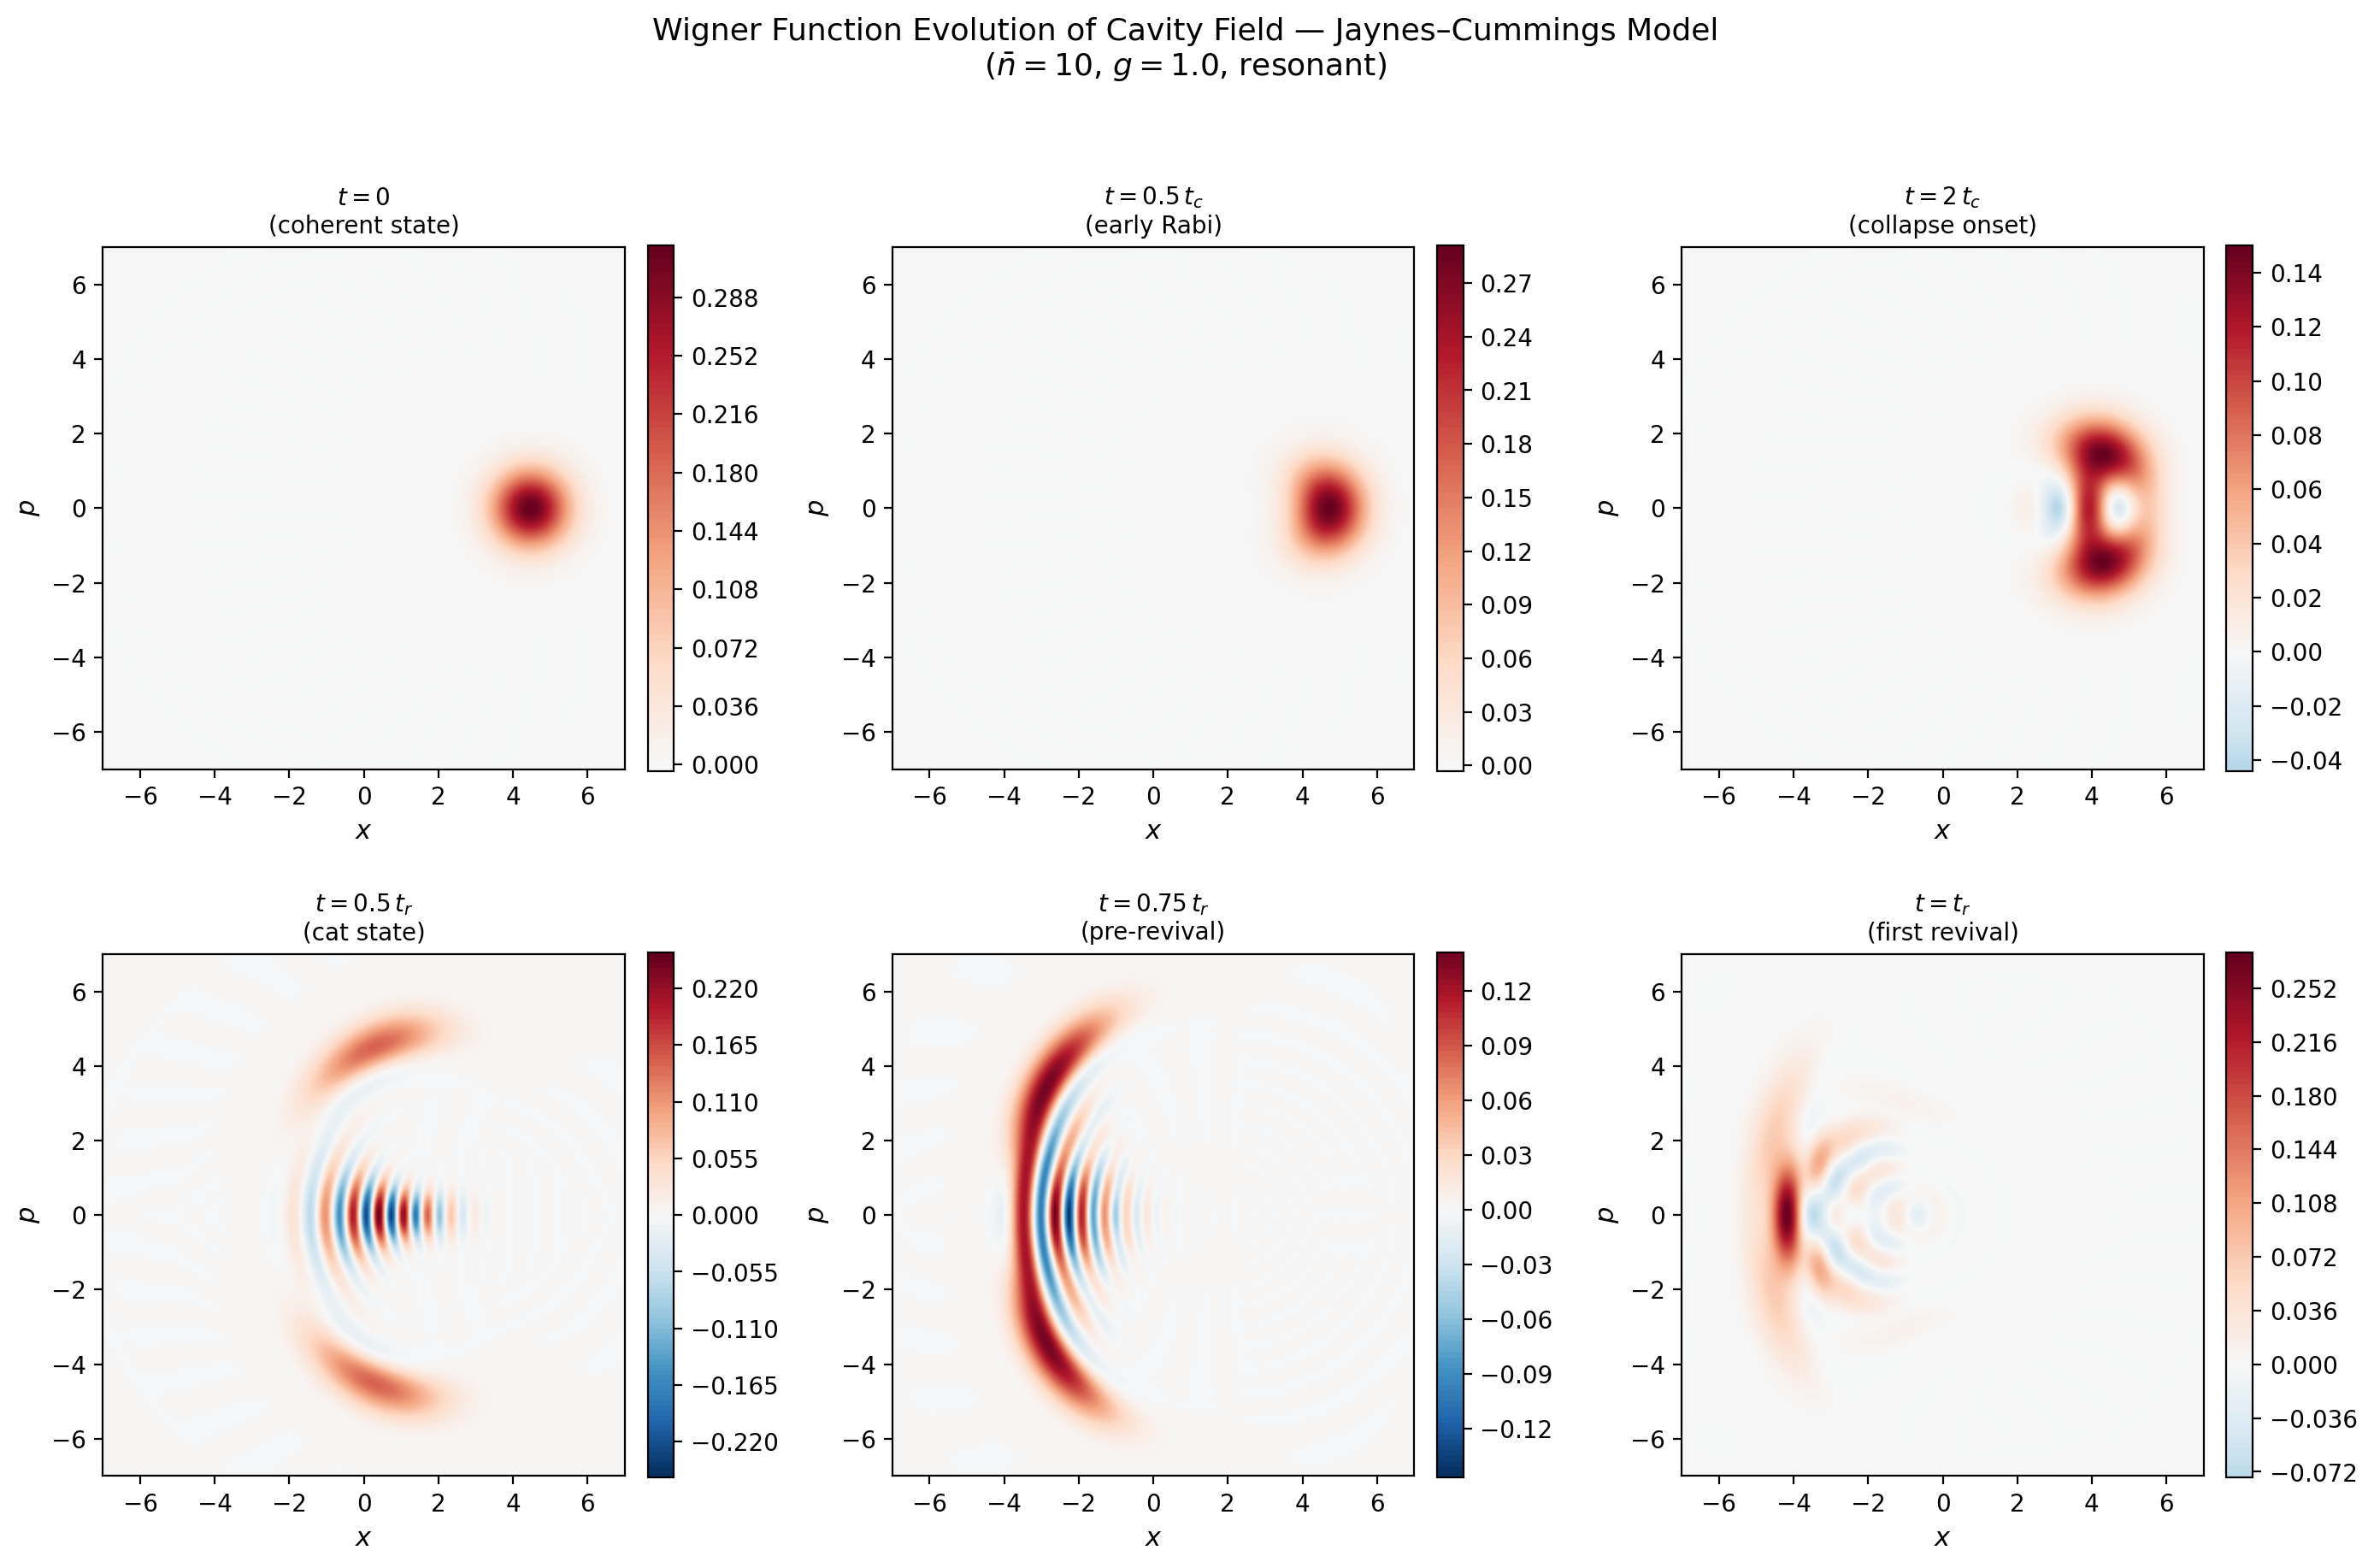
\includegraphics[width=\textwidth]{fig_wigner_evolution.png}
    \caption{Wigner function $W(x,p)$ of the reduced cavity field state at six characteristic times during Jaynes--Cummings evolution ($\bar{n} = 10$, $\Delta = 0$). At $t = 0$, the field is a coherent-state Gaussian. By $t = 2\,t_c$ (collapse onset), the distribution begins to spread. At $t = t_r/2$, a Schr\"{o}dinger cat state has formed: two distinct lobes connected by interference fringes with strong Wigner negativity ($\delta = 0.43$). By $t = t_r$, the field partially re-localizes at revival.}
    \label{fig:wigner_evolution}
\end{figure*}

\begin{figure*}[t]
    \centering
    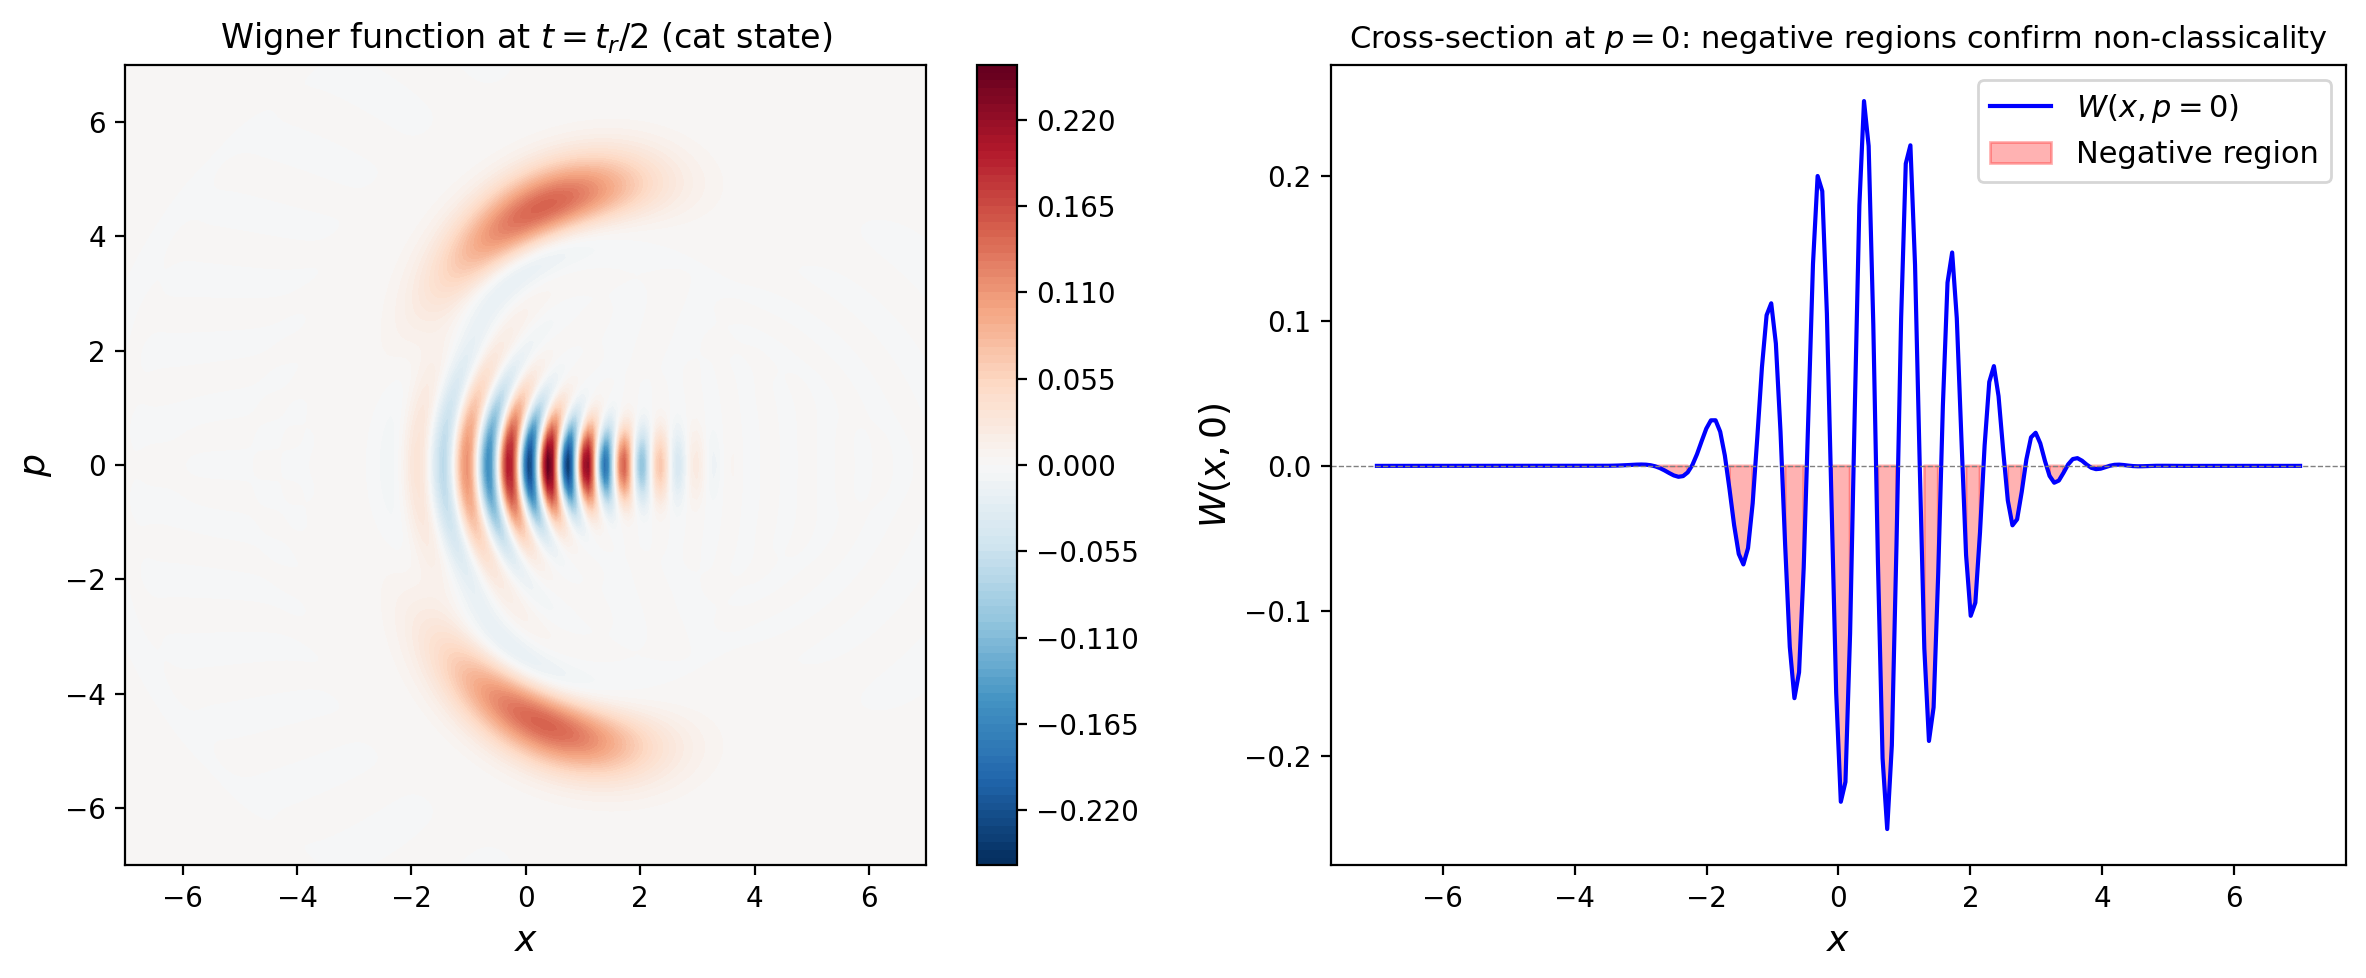
\includegraphics[width=\textwidth]{fig_cat_state_detail.png}
    \caption{Detailed view of the Schr\"{o}dinger cat state formed at $t = t_r/2$. Left: Wigner function contour plot showing two coherent-state lobes and interference fringes. Right: cross-section $W(x, p=0)$ with negative regions (shaded red) reaching $W \approx -0.22$. The negativity confirms the non-classical character of this dynamically generated state.}
    \label{fig:cat_detail}
\end{figure*}

\begin{figure*}[t]
    \centering
    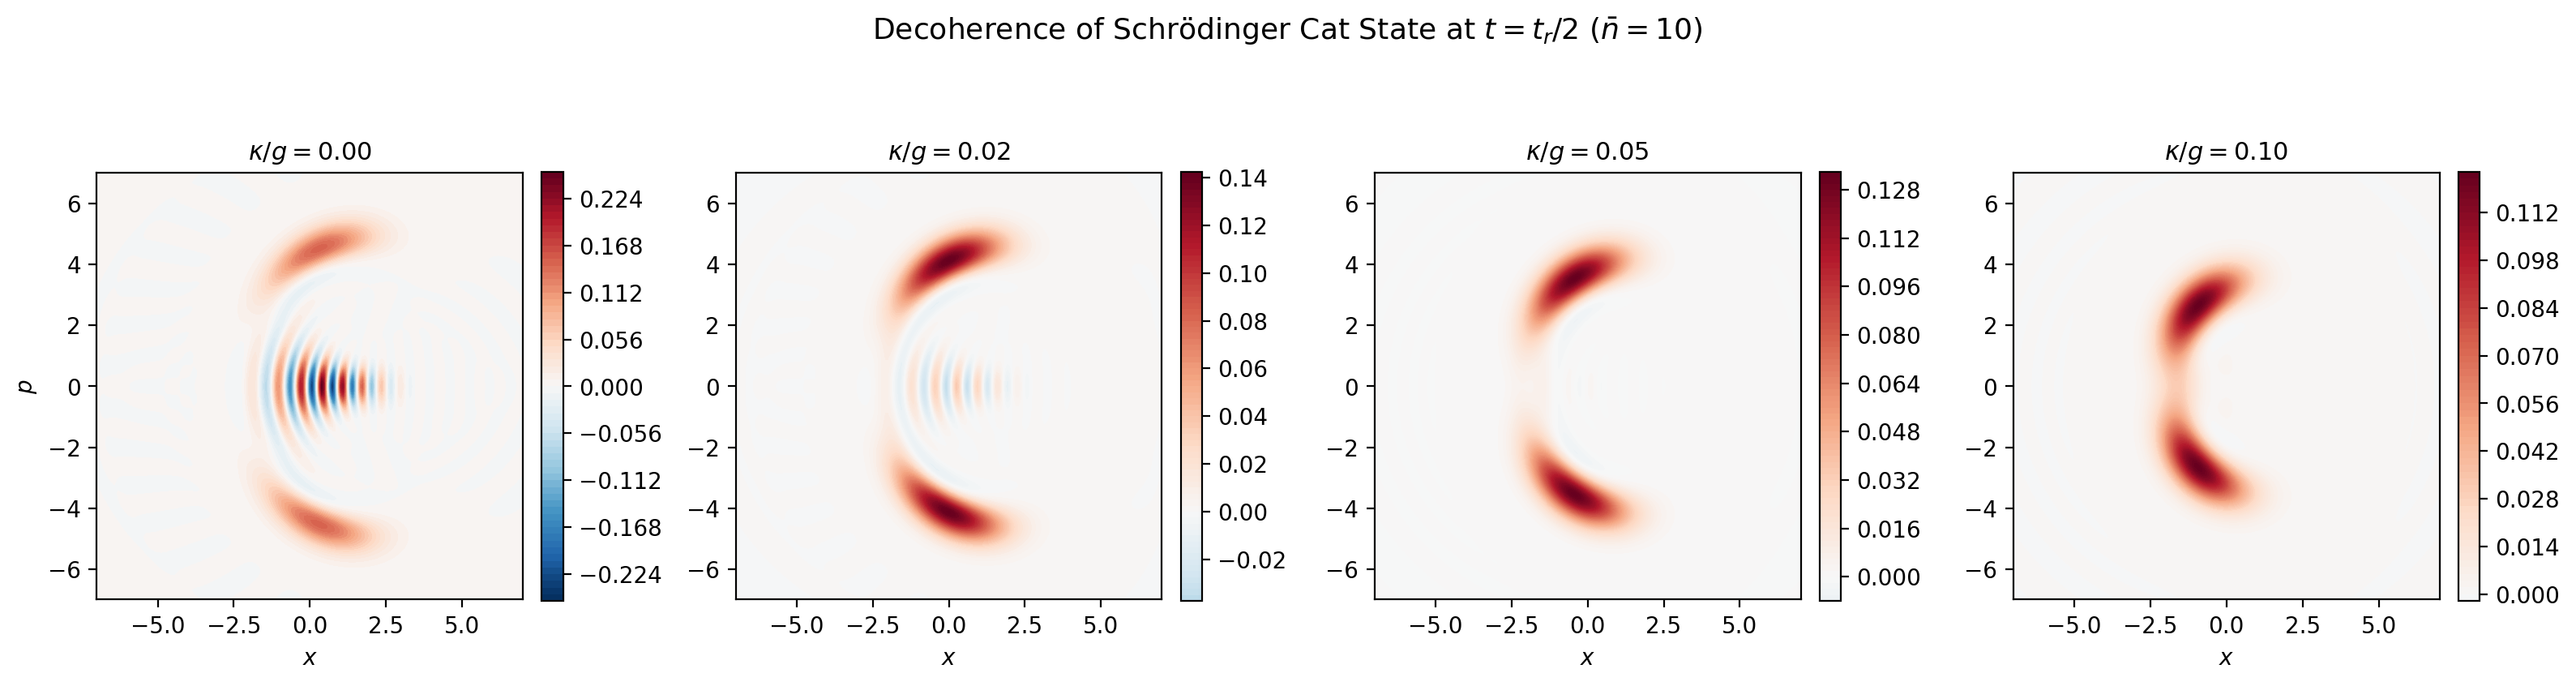
\includegraphics[width=\textwidth]{fig_wigner_decoherence.png}
    \caption{Decoherence of the Schr\"{o}dinger cat state. Wigner function at $t = t_r/2$ for increasing cavity decay rates $\kappa/g = 0,\, 0.02,\, 0.05,\, 0.10$ (left to right). The interference fringes are progressively destroyed; quantitative values of the Wigner negativity $\delta$ are given in Table~\ref{tab:decoherence}.}
    \label{fig:wigner_decoherence}
\end{figure*}

\begin{figure*}[t]
    \centering
    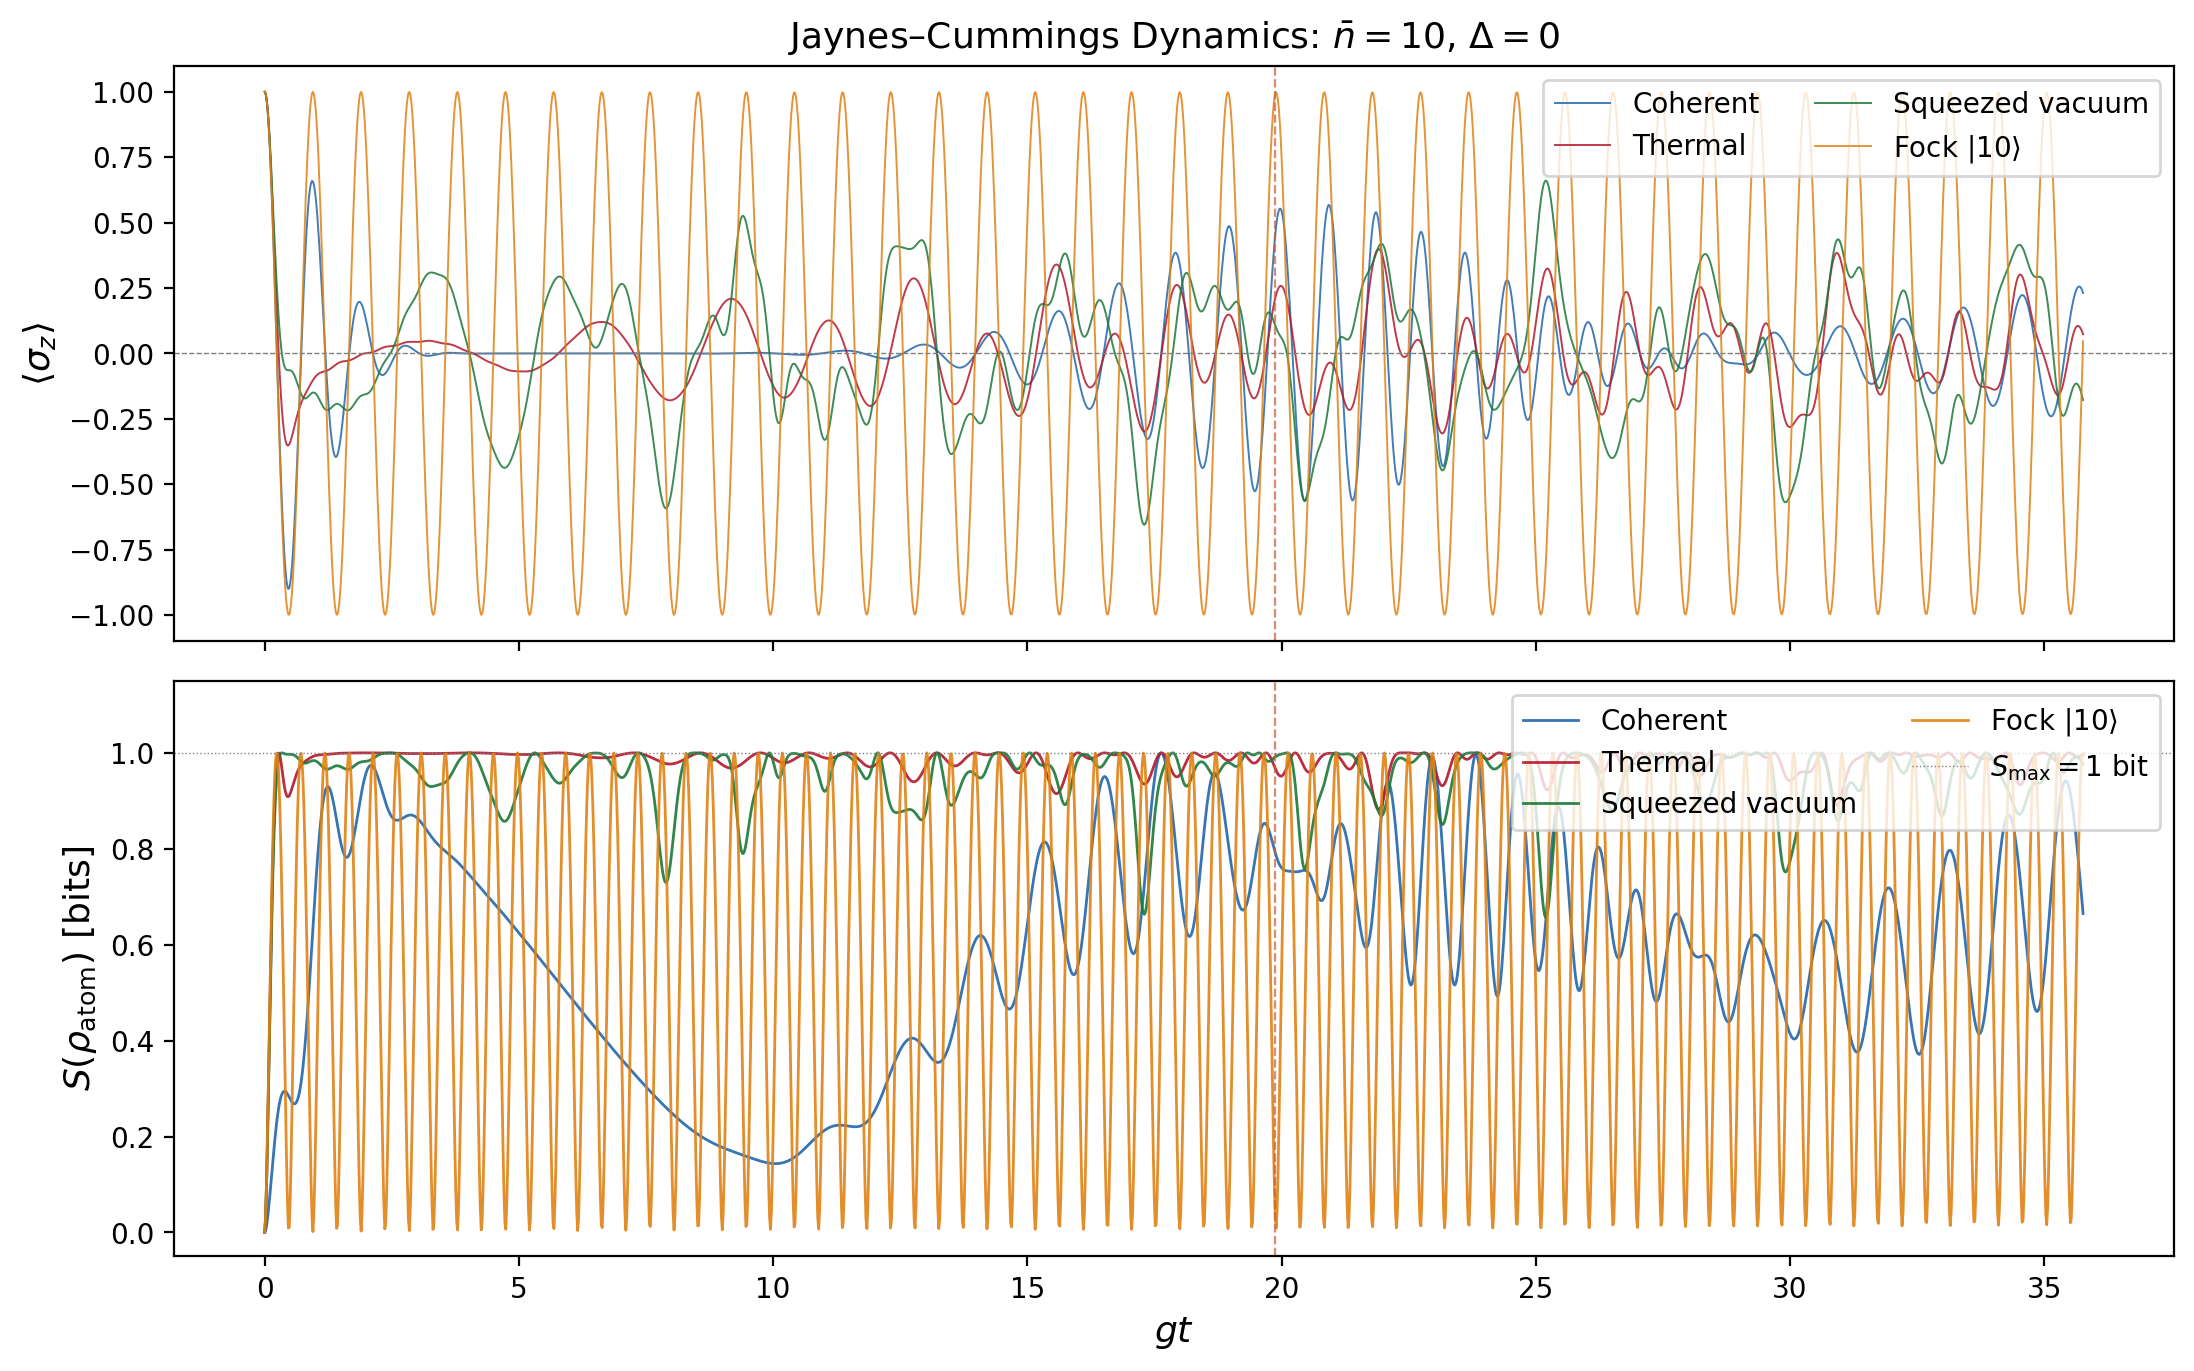
\includegraphics[width=\textwidth]{fig_entanglement_comparison.png}
    \caption{Comparison of Jaynes--Cummings dynamics for four initial field states with $\bar{n} = 10$. Top: atomic inversion $\langle\sigma_z\rangle$. Bottom: von Neumann entropy $S(\rho_{\text{atom}})$ of the reduced atomic state. The coherent state (blue) shows clean collapse-revival in both observables; the Fock state (orange) oscillates periodically; the thermal state (red) dephases irreversibly; the squeezed vacuum (green) shows intermediate behavior. The dashed purple line marks the revival time $t_r$.}
    \label{fig:entanglement_comparison}
\end{figure*}

\begin{figure}[t]
    \centering
    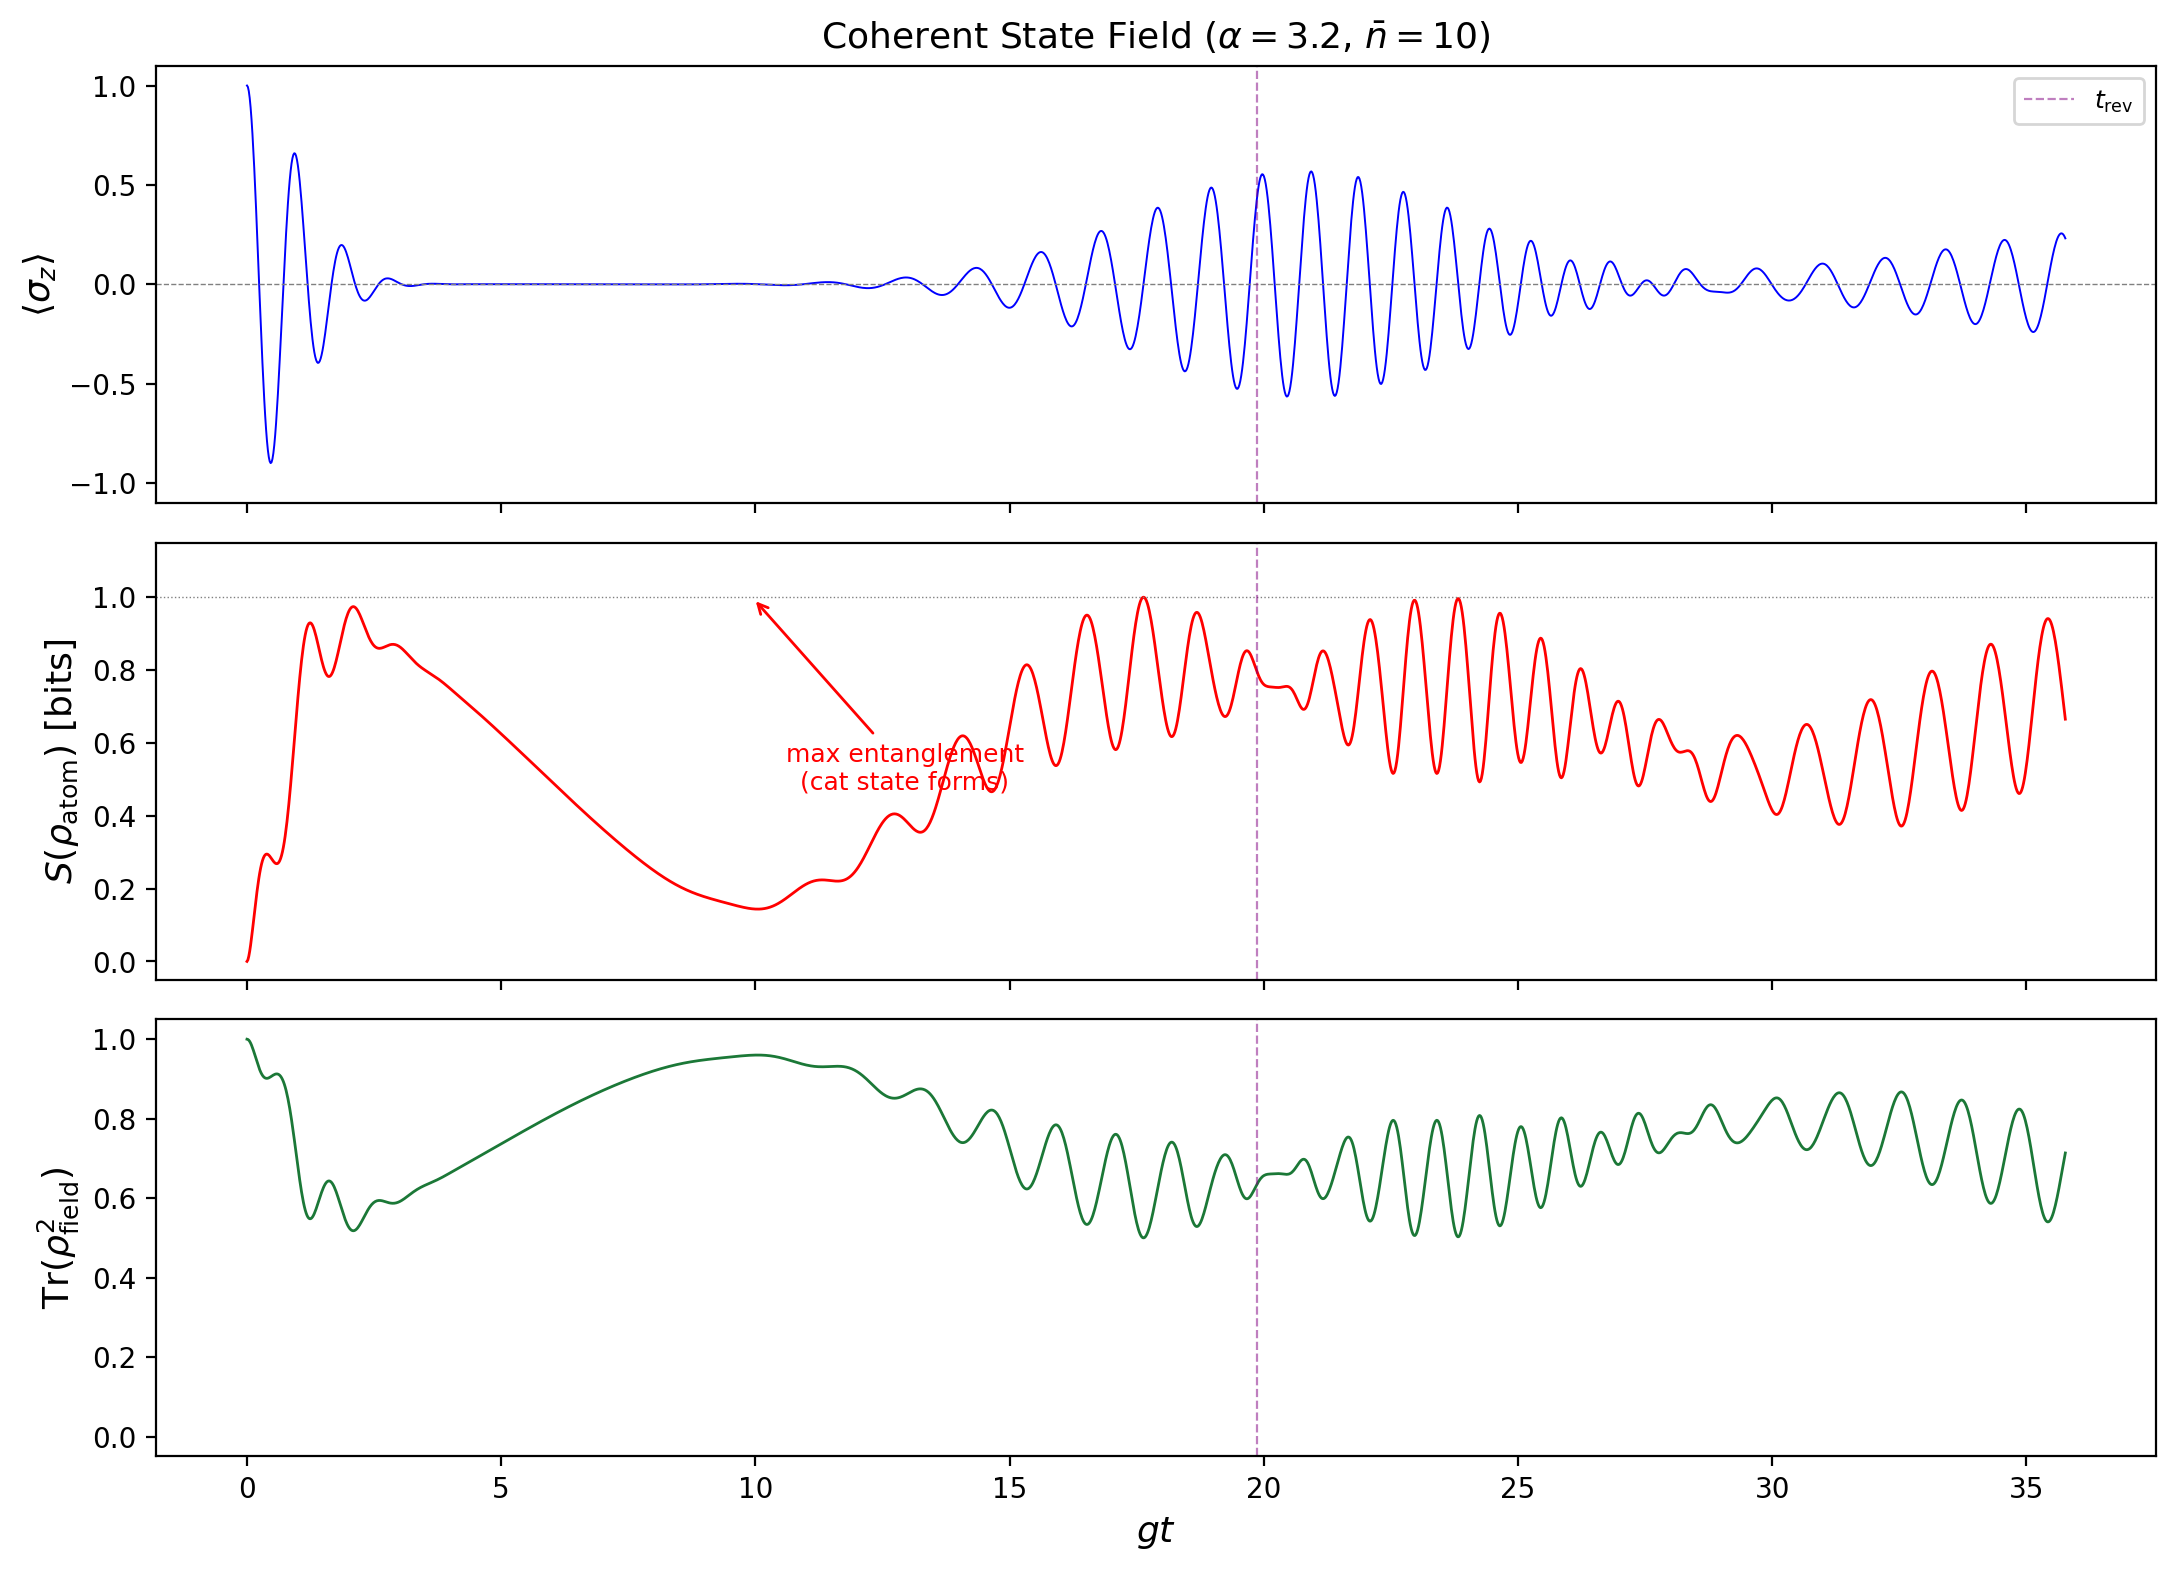
\includegraphics[width=\columnwidth]{fig_coherent_entropy_purity.png}
    \caption{Detailed coherent-state dynamics ($\bar{n} = 10$). Top: atomic inversion. Middle: entanglement entropy $S(\rho_{\text{atom}})$, peaking at $\approx 1$~bit during collapse and dipping at revival. Bottom: field purity $\mathcal{P} = \text{Tr}[\rho_{\text{field}}^2]$, reaching a minimum of $\approx 0.5$ during collapse (consistent with a two-component cat state). The dashed line marks $t_r$.}
    \label{fig:coherent_detail}
\end{figure}

\begin{figure*}[t]
    \centering
    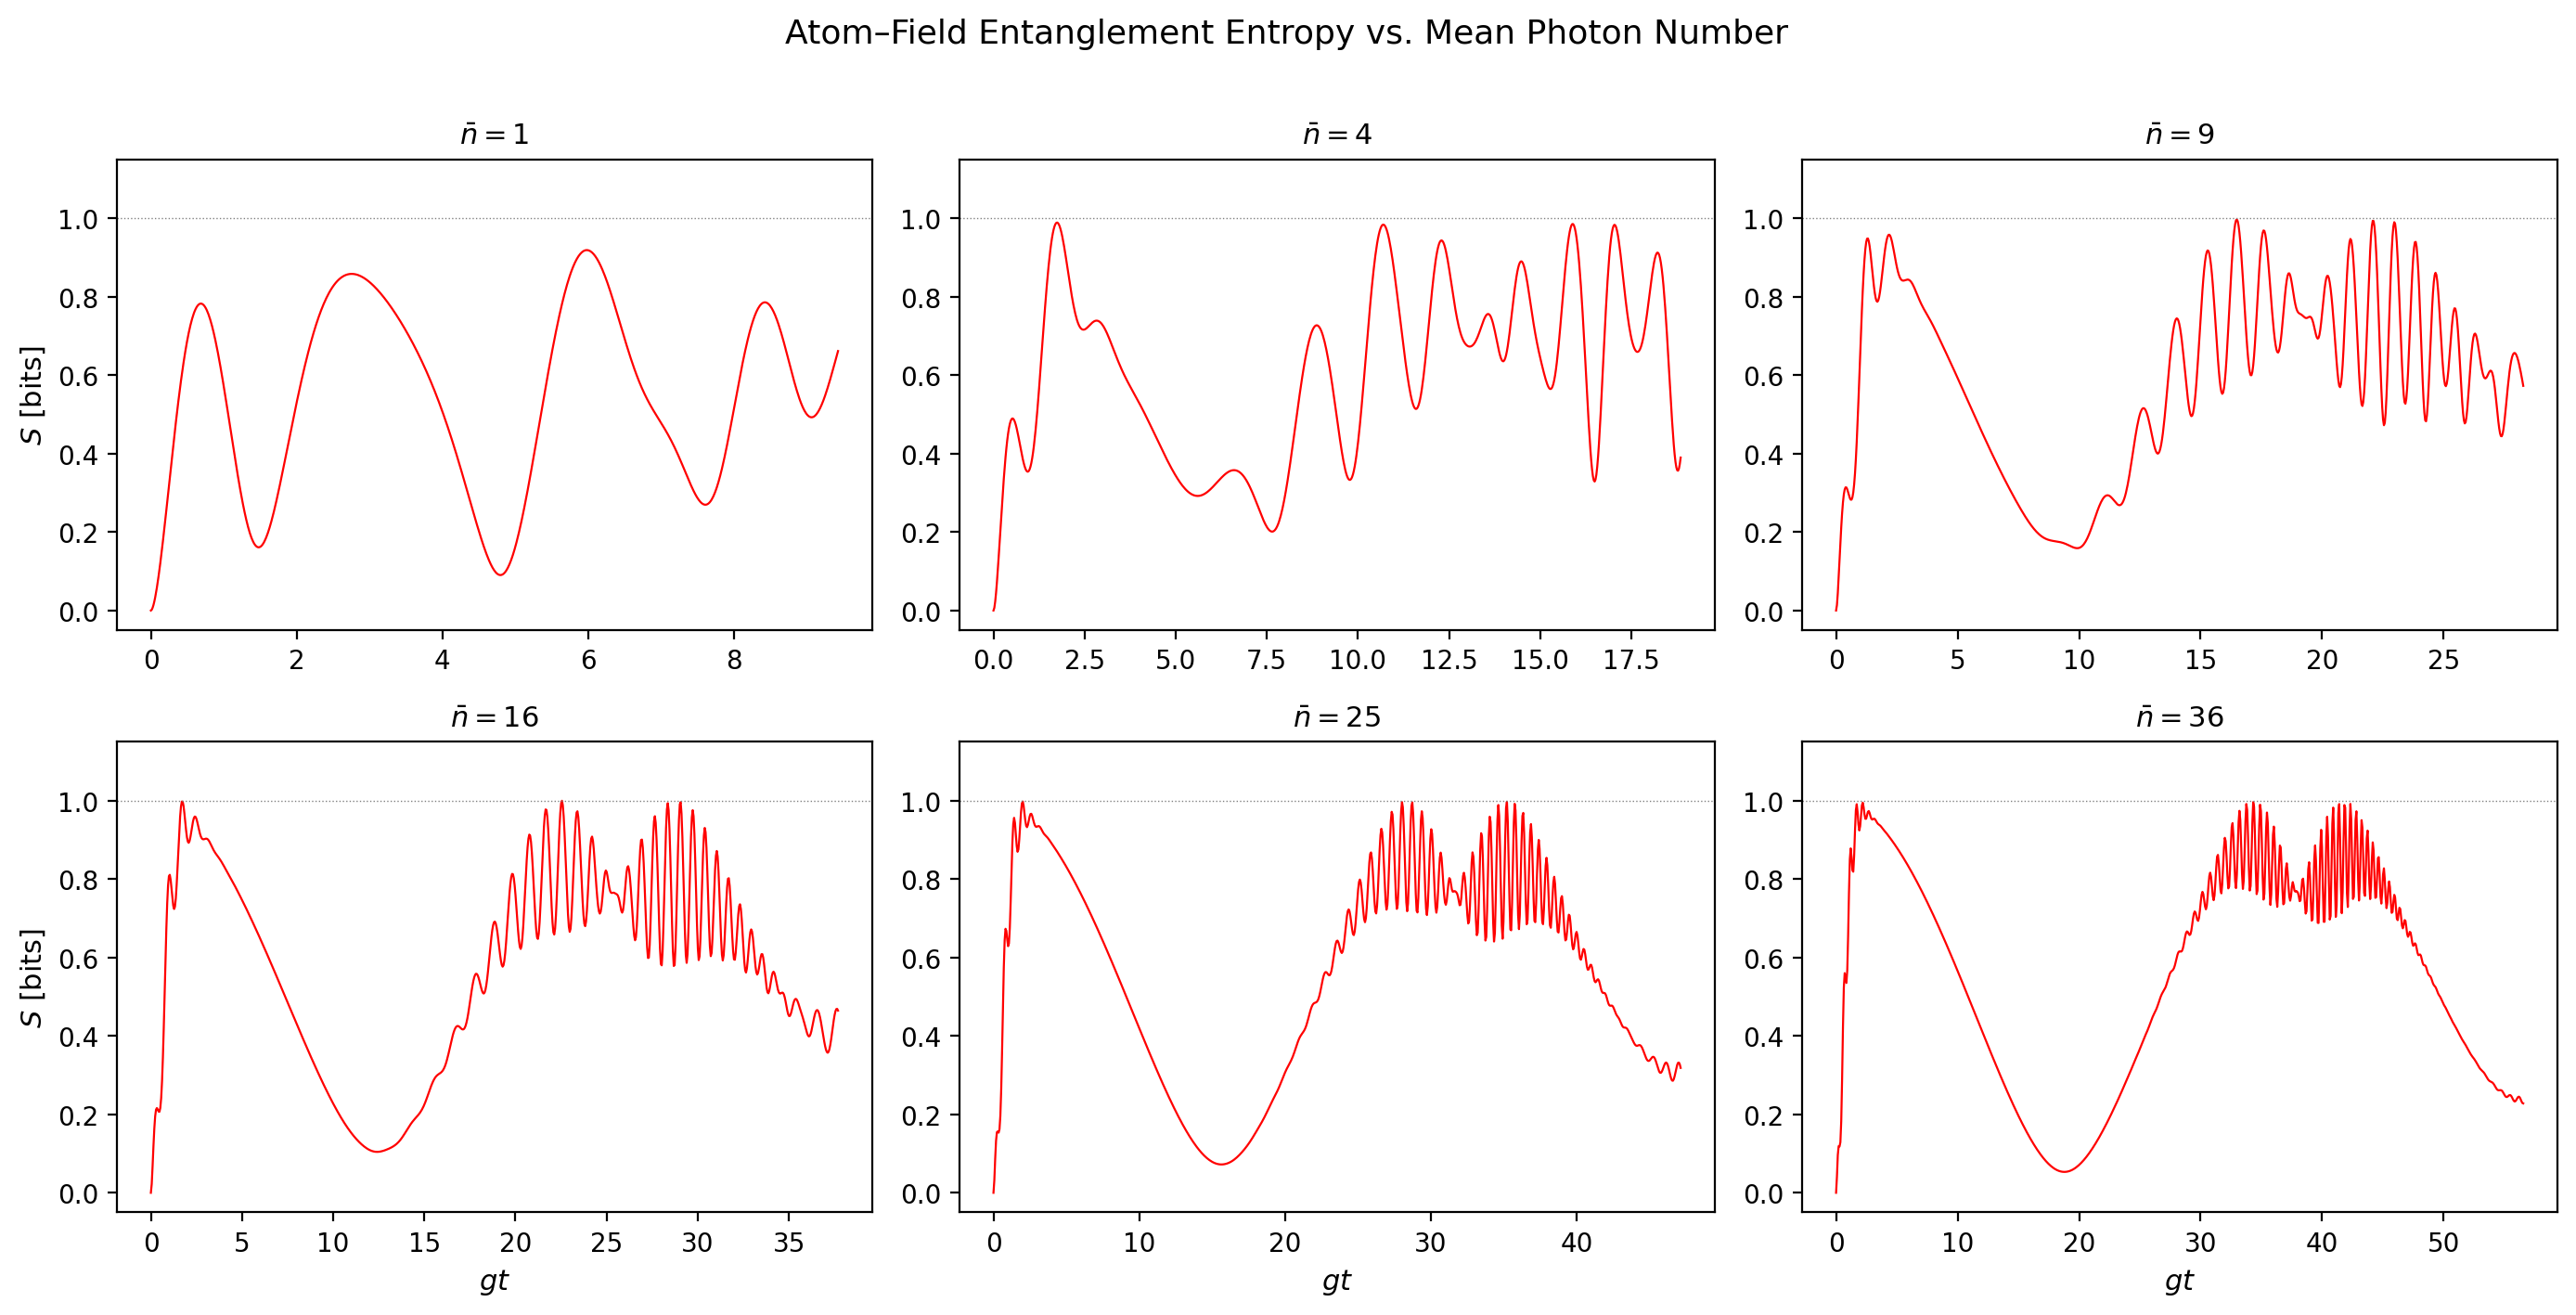
\includegraphics[width=\textwidth]{fig_entropy_nbar_scaling.png}
    \caption{Entanglement entropy $S(\rho_{\text{atom}})$ for coherent-state fields with $\bar{n} = 1,\, 4,\, 9,\, 16,\, 25,\, 36$. As $\bar{n}$ increases, the collapse time remains $\sim 1/g$ while the revival time grows as $t_r = 2\pi\sqrt{\bar{n}}/g$, producing a broader plateau of near-maximal entanglement. Clean revivals (entropy dips) emerge for $\bar{n} \gtrsim 9$.}
    \label{fig:entropy_nbar}
\end{figure*}

\begin{figure*}[t]
    \centering
    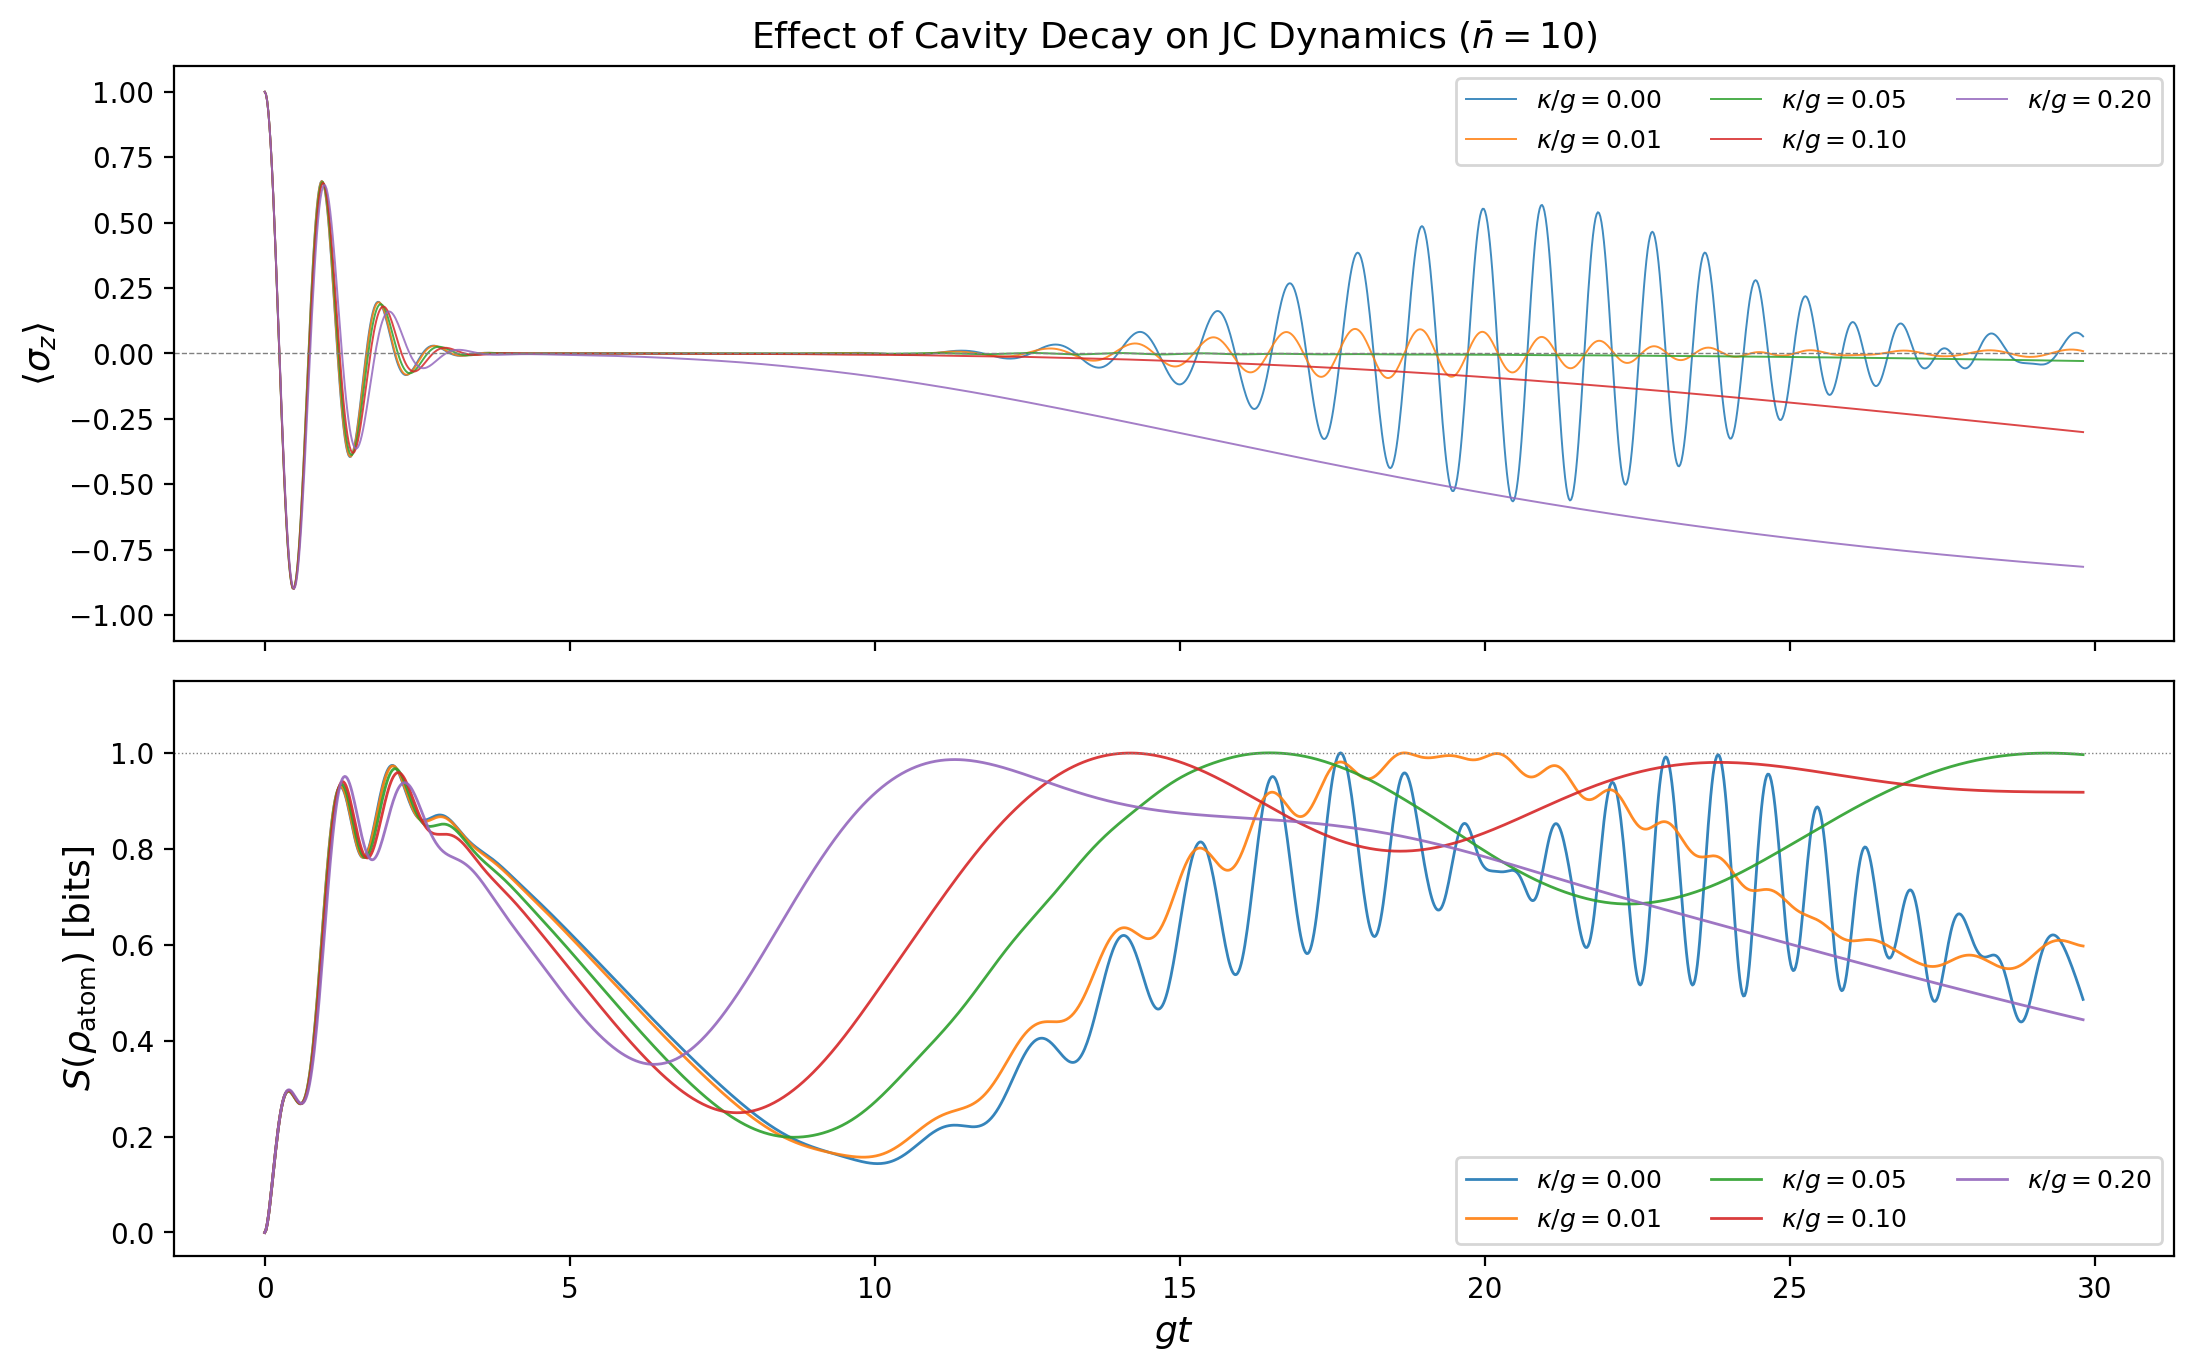
\includegraphics[width=\textwidth]{fig_dissipative_entanglement.png}
    \caption{Effect of cavity decay on JC dynamics ($\bar{n} = 10$). Top: atomic inversion for $\kappa/g = 0$--$0.20$. Bottom: entanglement entropy. Increasing $\kappa$ damps the Rabi oscillations, smears the revival feature in the entropy, and drives the system toward a mixed state.}
    \label{fig:dissipative_entropy}
\end{figure*}

% Original figures from the course paper, retained as supplementary
\begin{figure}[t]
    \centering
    
\includegraphics[width=\columnwidth]{jaynes_cummings_comparison.png}
    \caption{Atomic inversion for coherent (left) and thermal (right) field states at $\bar{n} = 4,\, 9,\, 14,\, 19,\, 24$. Coherent states show structured collapse-revival dynamics that sharpen with increasing $\bar{n}$; thermal states show rapid irreversible dephasing. Figure generated by Nguyen Khoi Nguyen, Boston University, 2024.}
    \label{fig:rabi_collapse_revival}
\end{figure}

\begin{figure}[t]
    \centering
    
\includegraphics[scale=0.35]{wigner_functions_3d.png}
    \caption{Static Wigner functions $W(x,p)$ for Fock states ($|0\rangle$, $|1\rangle$, $|6\rangle$, $|7\rangle$), squeezed vacuum ($r = 1.0$, $\phi = 0$ and $\pi/2$), and coherent states ($\alpha = 2$ and $2+2i$). Fock states exhibit ring-like structures and negativity; squeezed states show elliptical distributions; coherent states are displaced Gaussians with no negativity.}
    \label{fig:wigner_quantum_states}
\end{figure}

\begin{figure}[t]
    \centering
    
\includegraphics[scale=0.45]{wigner_functions_2d.png}
    \caption{Contour plots of the Wigner functions from Fig.~\ref{fig:wigner_quantum_states}. The color scale highlights negative regions (blue) as signatures of non-classicality.}
    \label{fig:wigner_2d_quantum_states}
\end{figure}

\begin{figure}[t]
    \centering
    
\includegraphics[scale=0.6]{mollow_triplet_driving_strength.png}
    \caption{Mollow triplet spectra for a driven two-level system at varying Rabi frequencies $\Omega/\gamma = 0.5$--$15$. As the driving strength increases, the single peak splits into three: a central Rayleigh line and two sidebands at $\omega - \omega_L = \pm\Omega$.}
    \label{fig:mollow_triplet}
\end{figure}


%% ============================================================
%% BIBLIOGRAPHY
%% ============================================================

\begin{thebibliography}{99}

\bibitem{rabi1937}
I.~I.~Rabi, Phys.\ Rev.\ \textbf{51}, 652 (1937).

\bibitem{scully1997}
M.~O.~Scully and M.~S.~Zubairy, \textit{Quantum Optics} (Cambridge University Press, 1997).

\bibitem{allen1975}
L.~Allen and J.~H.~Eberly, \textit{Optical Resonance and Two-Level Atoms} (Dover, 1975).

\bibitem{gerry2004}
C.~C.~Gerry and P.~L.~Knight, \textit{Introductory Quantum Optics} (Cambridge University Press, 2004).

\bibitem{jaynes1963}
E.~T.~Jaynes and F.~W.~Cummings, Proc.\ IEEE \textbf{51}, 89 (1963).

\bibitem{eberly1980}
J.~H.~Eberly, N.~B.~Narozhny, and J.~J.~Sanchez-Mondragon, Phys.\ Rev.\ Lett.\ \textbf{44}, 1323 (1980).

\bibitem{brune1996}
M.~Brune, E.~Hagley, J.~Dreyer, X.~Ma\^{i}tre, A.~Maali, C.~Wunderlich, J.~M.~Raimond, and S.~Haroche, Phys.\ Rev.\ Lett.\ \textbf{77}, 4887 (1996).

\bibitem{rempe1987}
G.~Rempe, H.~Walther, and N.~Klein, Phys.\ Rev.\ Lett.\ \textbf{58}, 353 (1987).

\bibitem{haroche2006}
S.~Haroche and J.-M.~Raimond, \textit{Exploring the Quantum: Atoms, Cavities, and Photons} (Oxford University Press, 2006).

\bibitem{blais2021}
A.~Blais, A.~L.~Grimsmo, S.~M.~Girvin, and A.~Wallraff, Rev.\ Mod.\ Phys.\ \textbf{93}, 025005 (2021).

\bibitem{glauber1963}
R.~J.~Glauber, Phys.\ Rev.\ \textbf{131}, 2766 (1963).

\bibitem{sudarshan1963}
E.~C.~G.~Sudarshan, Phys.\ Rev.\ Lett.\ \textbf{10}, 277 (1963).

\bibitem{aasi2013}
J.~Aasi \textit{et al.}\ (LIGO Scientific Collaboration), Nat.\ Photonics \textbf{7}, 613 (2013).

\bibitem{tse2019}
M.~Tse \textit{et al.}\ (LIGO Scientific Collaboration), Phys.\ Rev.\ Lett.\ \textbf{123}, 231107 (2019).

\bibitem{wigner1932}
E.~Wigner, Phys.\ Rev.\ \textbf{40}, 749 (1932).

\bibitem{hudson1974}
R.~L.~Hudson, Rep.\ Math.\ Phys.\ \textbf{6}, 249 (1974).

\bibitem{kenfack2004}
A.~Kenfack and K.~\.{Z}yczkowski, J.~Opt.~B: Quantum Semiclass.\ Opt.\ \textbf{6}, 396 (2004).

\bibitem{mollow1969}
B.~R.~Mollow, Phys.\ Rev.\ \textbf{188}, 1969 (1969).

\bibitem{thompson1992}
R.~J.~Thompson, G.~Rempe, and H.~J.~Kimble, Phys.\ Rev.\ Lett.\ \textbf{68}, 1132 (1992).

\bibitem{lindblad1976}
G.~Lindblad, Commun.\ Math.\ Phys.\ \textbf{48}, 119 (1976).

\bibitem{wiseman2009}
H.~M.~Wiseman and G.~J.~Milburn, \textit{Quantum Measurement and Control} (Cambridge University Press, 2009).

\bibitem{zurek2003}
W.~H.~Zurek, Rev.\ Mod.\ Phys.\ \textbf{75}, 715 (2003).

\bibitem{nielsen2000}
M.~A.~Nielsen and I.~L.~Chuang, \textit{Quantum Computation and Quantum Information} (Cambridge University Press, 2000).

\bibitem{phoenix1988}
S.~J.~D.~Phoenix and P.~L.~Knight, Ann.\ Phys.\ (N.Y.) \textbf{186}, 381 (1988).

\bibitem{johansson2012}
J.~R.~Johansson, P.~D.~Nation, and F.~Nori, Comp.\ Phys.\ Comm.\ \textbf{183}, 1760 (2012).

\bibitem{johansson2013}
J.~R.~Johansson, P.~D.~Nation, and F.~Nori, Comp.\ Phys.\ Comm.\ \textbf{184}, 1234 (2013).

\bibitem{gea-banacloche1990}
J.~Gea-Banacloche, Phys.\ Rev.\ Lett.\ \textbf{65}, 3385 (1990).

\bibitem{kimble1977}
H.~J.~Kimble, M.~Dagenais, and L.~Mandel, Phys.\ Rev.\ Lett.\ \textbf{39}, 691 (1977).

\bibitem{ekert1991}
A.~K.~Ekert, Phys.\ Rev.\ Lett.\ \textbf{67}, 661 (1991).

\bibitem{hofheinz2009}
M.~Hofheinz, H.~Wang, M.~Ansmann, R.~C.~Bialczak, E.~Lucero, M.~Neeley, A.~D.~O'Connell, D.~Sank, J.~Wenner, J.~M.~Martinis, and A.~N.~Cleland, Nature \textbf{459}, 546 (2009).

\bibitem{ofek2016}
P.~Ofek \textit{et al.}, Nature \textbf{536}, 441 (2016).

\bibitem{walls2008}
D.~F.~Walls and G.~J.~Milburn, \textit{Quantum Optics}, 2nd ed.\ (Springer, 2008).

\end{thebibliography}

\end{document}
